\chapter{Implementazione Sperimentale e Risultati}
\label{cap:implementazione_sperimentale_risultati}

Questo capitolo descrive l'implementazione software del sistema presentato nel Capitolo~\ref{cap:architettura_sistema_metodologia} e riporta i risultati sperimentali ottenuti applicando la metodologia descritta ai tre dataset selezionati (Breast Cancer Wisconsin, Wine, Digits). Vengono presentati, in ordine: la configurazione dell'ambiente containerizzato, l'implementazione dei moduli della pipeline (acquisizione, preprocessing, codifica quantistica, addestramento, esecuzione, valutazione), la configurazione sperimentale specifica adottata per ciascun modello, i risultati ottenuti per ciascun dataset a confronto tra modelli classici e quantistici, un'analisi comparativa trasversale, e infine una discussione critica dei risultati alla luce dei limiti metodologici e computazionali discussi nei capitoli precedenti.

\begin{quote}
\textit{Nota metodologica: la campagna sperimentale è stata completata in simulazione ideale e in simulazione con modello di rumore per tutti e tre i dataset; i valori riportati in queste condizioni sono risultati reali. L'esecuzione su hardware quantistico reale non è invece stata completata entro i tempi e le risorse disponibili per questo lavoro, per i motivi documentati nella Sezione~\ref{sec:limiti_studio}; le tabelle relative a questa modalità riportano una nota esplicita al posto dei valori numerici.}
\end{quote}

\section{Struttura del progetto e ambiente containerizzato}
\label{sec:struttura_progetto}

\subsection{Organizzazione del repository}
Il codice sorgente sviluppato per questo lavoro è organizzato secondo la struttura modulare anticipata nella Sezione~\ref{sec:architettura_generale}, con una separazione netta tra codice riutilizzabile (pacchetto \texttt{src}), notebook di sperimentazione (\texttt{notebooks}), dati intermedi (\texttt{data}) e configurazione dell'ambiente (file \texttt{Dockerfile} e \texttt{docker-compose.yml}):

\begin{verbatim}
experiments/
|-- Dockerfile
|-- docker-compose.yml
|-- requirements.txt
|-- config.py
|-- run_pipeline.py
|-- data/
|   |-- raw/
|   |-- processed/
|-- notebooks/
|   |-- 01_data_acquisition.ipynb
|   |-- ...
|-- src/
|   |-- pipeline.py
|   |-- data/
|   |   |-- acquisition.py
|   |   `-- preprocessing.py
|   ...
|-- results/
    |-- figures/
    |-- tables/
\end{verbatim}

Questa organizzazione consente di importare le funzioni implementate nel pacchetto \texttt{src} sia dai notebook di sperimentazione sia da eventuali script di automazione, evitando la duplicazione di codice tra le diverse fasi della pipeline.

Il file \texttt{config.py} centralizza gli iperparametri sperimentali specifici di ciascun dataset (numero di componenti PCA, ripetizioni della feature map e dell'ansatz, numero massimo di iterazioni dell'ottimizzatore) riportati in Tabella~\ref{tab:configurazione_completa}, oltre ai parametri di sottocampionamento e di suddivisione in chunk usati dalle modalità di esecuzione più realistiche (\texttt{HARDWARE\_TRAIN\_SAMPLE\_SIZE}, 
\linebreak\texttt{HARDWARE\_TEST\_SAMPLE\_SIZE}, \texttt{QSVC\_MAX\_CIRCUITS\_PER\_JOB}, Sezione~\ref{sec:esecuzione_hardware_reale}) e alla dimensione dei chunk per il QSVC in simulazione ideale 
\linebreak(\texttt{QSVC\_IDEAL\_MAX\_CIRCUITS\_PER\_JOB}, si veda la Sezione "Limiti dello studio e minacce alla validità"), in modo che notebook e script di automazione facciano riferimento a un'unica fonte di verità. Lo script \texttt{run\_pipeline.py} è un orchestratore da riga di comando: la logica di addestramento, valutazione e produzione delle figure si trova nel modulo \texttt{src/pipeline.py} (Sezione~\ref{sec:impl_orchestrazione}) e nel modulo \texttt{src/evaluation/plots.py}, da cui \texttt{run\_pipeline.py} importa senza duplicarne il contenuto, in modo che la stessa logica sia riutilizzabile dai notebook di sperimentazione. Lo script accetta il flag \texttt{--datasets}, che consente di eseguire la pipeline completa (acquisizione, preprocessing, addestramento dei modelli classici con grid search, addestramento di QSVC e VQC in simulazione ideale, valutazione) su un sottoinsieme di dataset alla volta, anche un singolo dataset per singola invocazione, utile data la durata non trascurabile dell'addestramento del QSVC sui dataset più grandi, e il flag \texttt{--aggregate}, che ricalcola le tabelle e le figure comparative trasversali (Sezione~\ref{sec:analisi_comparativa}) a partire dai risultati per dataset già presenti in \texttt{results/tables}, anche parziali; un risultato equivalente si ottiene, in modo interattivo, dal notebook \texttt{07\_results\_comparison.ipynb} (Sezione~\ref{sec:impl_orchestrazione}). Due ulteriori flag opzionali eseguono analisi supplementari a partire dagli stessi dati preprocessati: \texttt{--digits-pca-sensitivity}, che riproduce l'analisi di sensitività del QSVC al numero di componenti PCA sul dataset Digits (Tabella~\ref{tab:digits_sensitivity_pca}, Sezione~\ref{sec:risultati_digits}), e \texttt{--optimizer-comparison}, che confronta gli ottimizzatori COBYLA e SPSA per il VQC sul dataset Breast Cancer Wisconsin (Tabella~\ref{tab:confronto_ottimizzatori}, Sezione~\ref{sec:confronto_ottimizzatori}). Il codice sorgente completo è disponibile nella cartella \texttt{experiments/} del repository della tesi\footnote{\url{https://github.com/rosario-cafaro/l8-thesis}.}.

\subsection{Dockerfile}
\label{sec:implementazione_dockerfile}

Il file \texttt{Dockerfile}, la cui struttura generale è stata anticipata nella Sezione~\ref{sec:docker}, definisce l'immagine utilizzata per tutti gli esperimenti riportati in questo capitolo:

\lstinputlisting[language={}]{experiments/Dockerfile}

Il file \texttt{requirements.txt} associato fissa le versioni esatte delle librerie utilizzate, in coerenza con quanto discusso nella Sezione~\ref{sec:docker} riguardo alla necessità di garantire la riproducibilità a fronte del ritmo di aggiornamento rapido di Qiskit. L'immagine di base è stata fissata a Python 3.12 anziché a una versione precedente poiché le versioni di NumPy e Pandas effettivamente validate nell'ambiente di sviluppo richiedono Python 3.12 o superiore:

\lstinputlisting[language={}]{experiments/requirements.txt}

\subsection{docker-compose.yml}
\label{sec:docker_compose}
Il file \texttt{docker-compose.yml} orchestra il servizio definito dal Dockerfile, secondo lo schema descritto nella Sezione~\ref{sec:docker} e illustrato in Figura~\ref{fig:docker_architettura}:

\lstinputlisting[language={}]{experiments/docker-compose.yml}

Il token di accesso a IBM Quantum Platform, necessario non solo per l'esecuzione su hardware reale descritta nella Sezione~\ref{sec:esecuzione_hardware_reale} ma anche per la sola modalità \texttt{noisy\_simulation} (Sezione~\ref{sec:impl_backend}), che pur eseguendo i circuiti localmente richiede una connessione autenticata al servizio per scaricare i dati di calibrazione di un backend reale, viene iniettato tramite variabile d'ambiente a partire da un file \texttt{.env} non incluso nel controllo di versione, per evitare di esporre credenziali personali nel repository del progetto.

\begin{figure}[htbp]
    \centering
    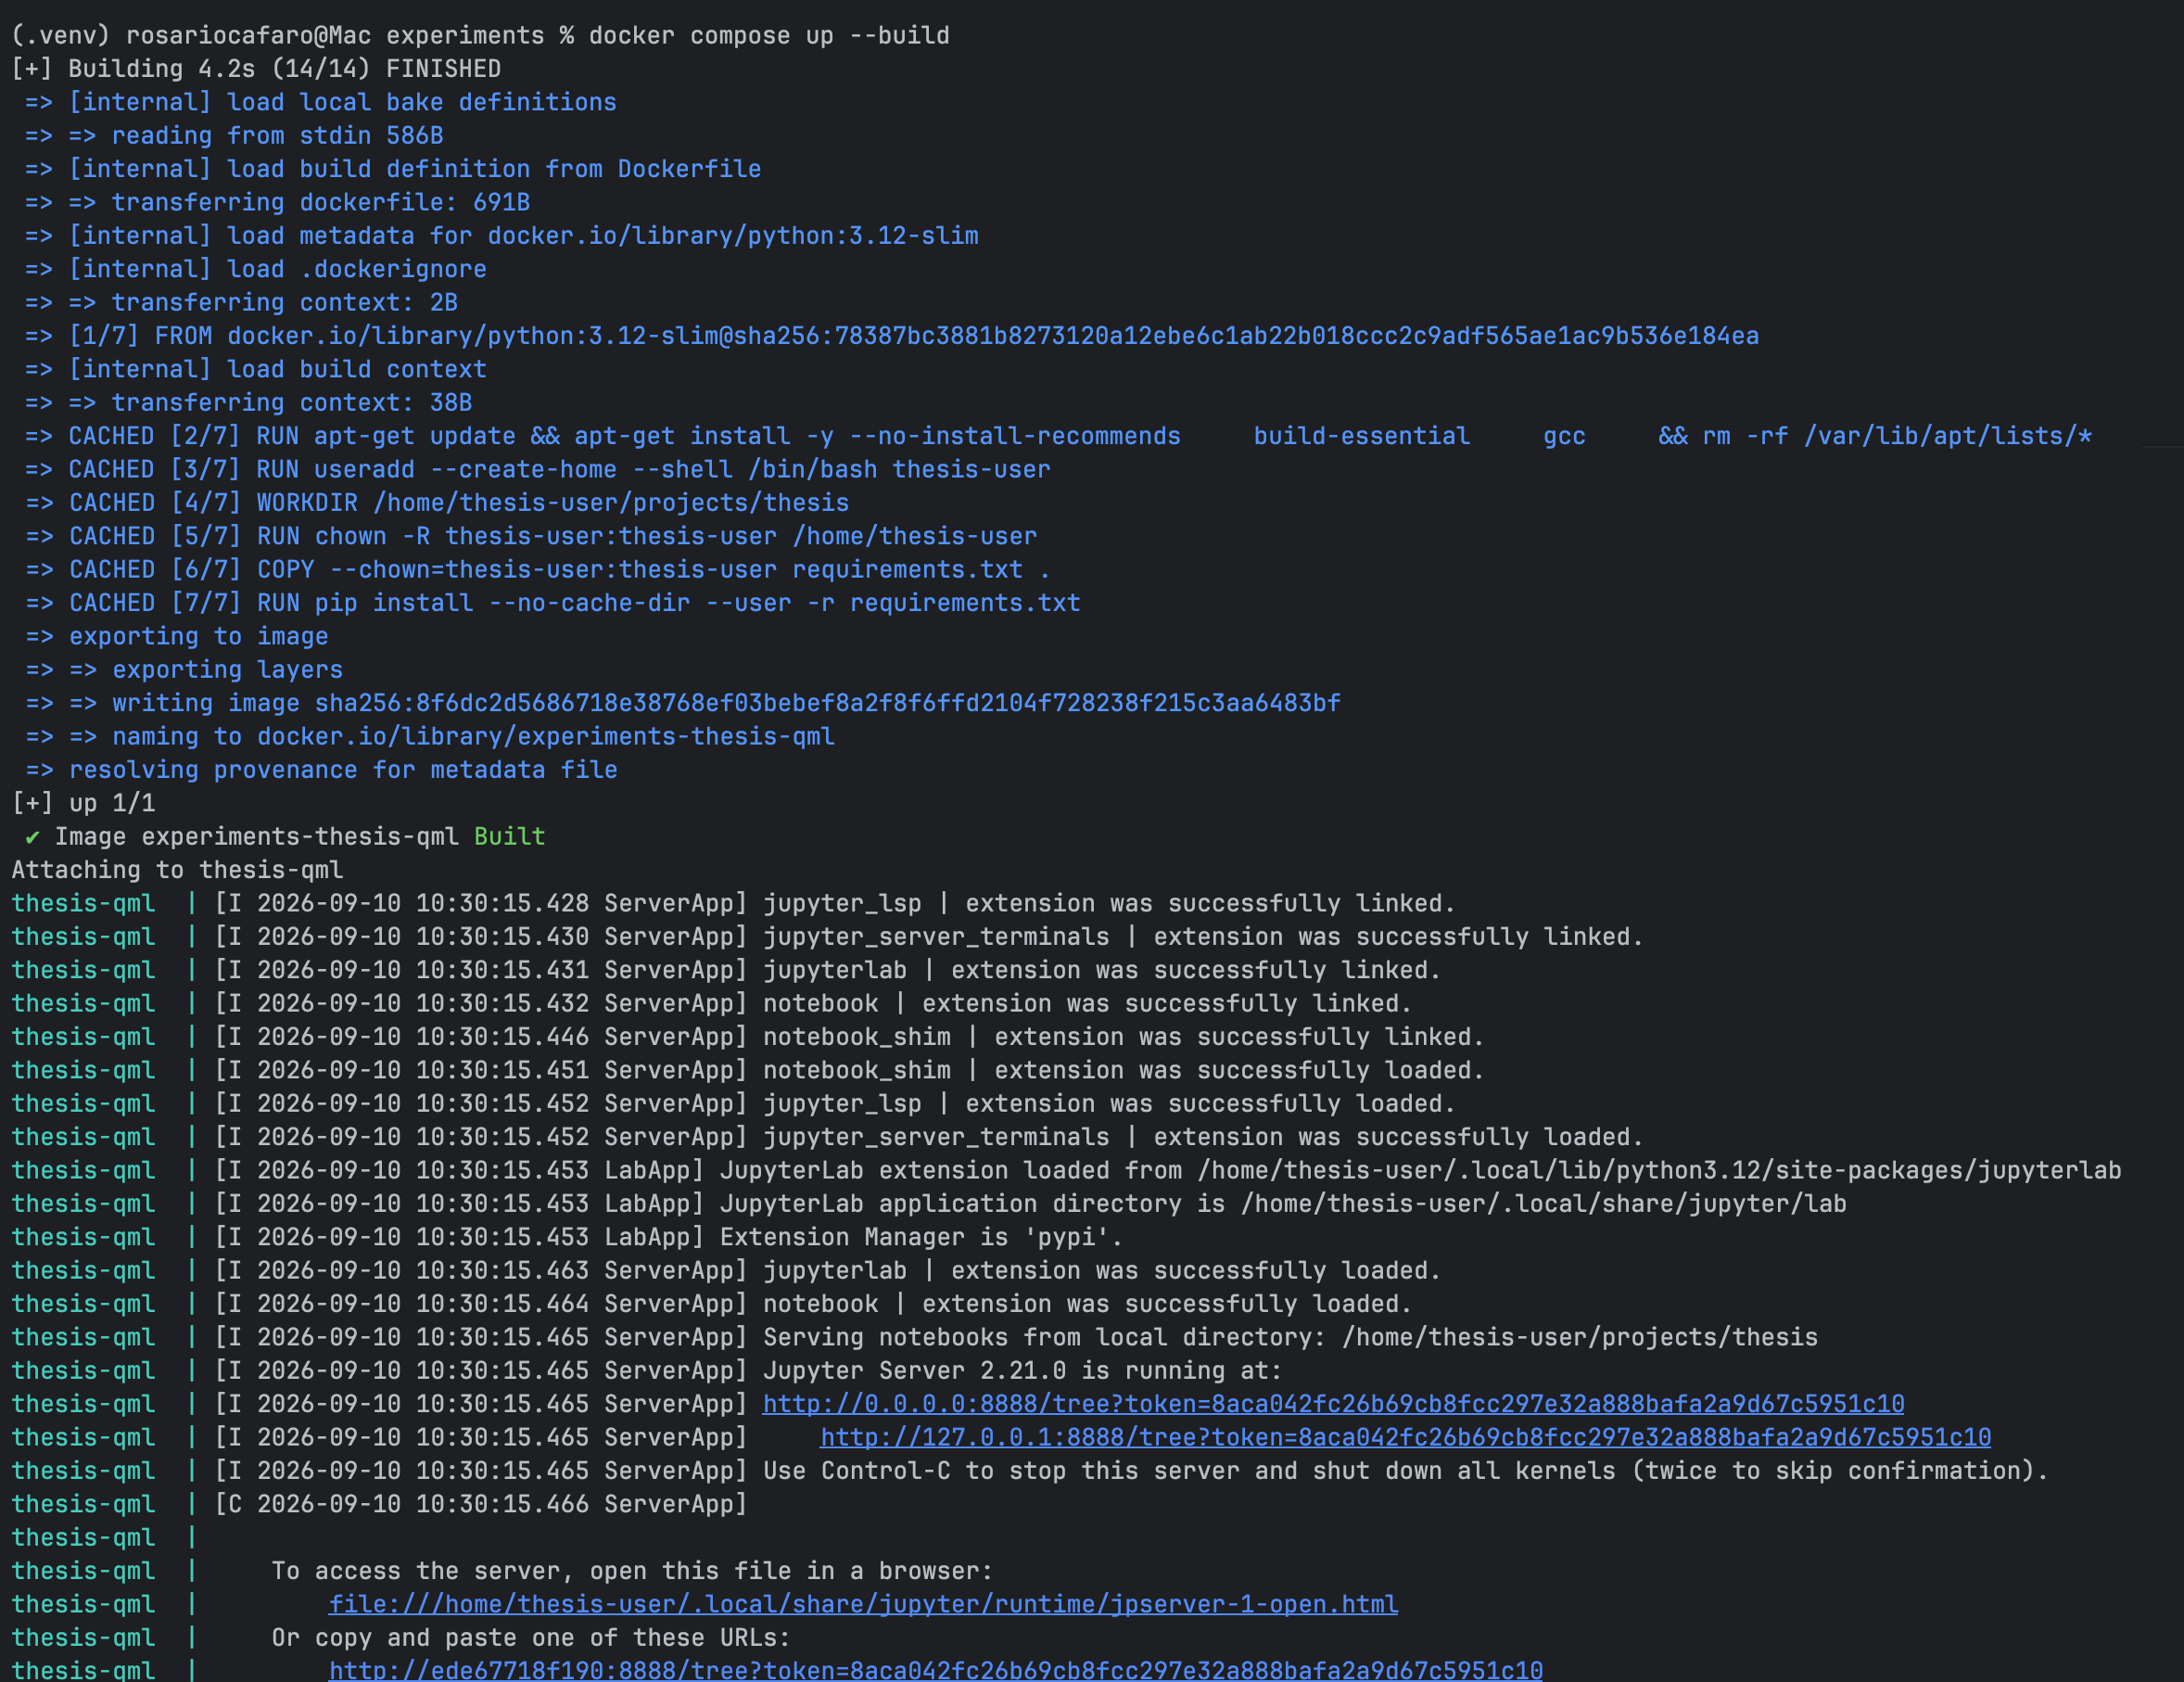
\includegraphics[width=0.70\textwidth]{assets/docker_compose_up.png}
    \caption{Avvio dell'ambiente containerizzato tramite Docker Compose.}
    \label{fig:screenshot_docker_up}
\end{figure}

\section{Implementazione dei moduli della pipeline}
\label{sec:implementazione_moduli}

\subsection{Acquisizione e validazione dei dati}
\label{sec:impl_acquisizione}

Il modulo di acquisizione, corrispondente al primo blocco dell'architettura descritta nella Sezione~\ref{sec:architettura_generale}, carica i tre dataset tramite le funzioni dedicate di Scikit-learn ed esegue una validazione preliminare:

\lstinputlisting[language=Python]{experiments/src/data/acquisition.py}

I risultati della validazione preliminare per i tre dataset sono riassunti in Tabella~\ref{tab:validazione_dataset}, e confermano l'assenza di valori mancanti e la natura interamente numerica delle feature, come anticipato nella Sezione~\ref{sec:dataset_preprocessing}.

\begin{table}[htbp]
\centering
\caption{Esito della validazione preliminare dei tre dataset.}
\label{tab:validazione_dataset}
\small
\setlength{\tabcolsep}{4pt}
\begin{tabular}{lccccc}
\toprule
\textbf{Dataset} & \textbf{Campioni} & \textbf{Feature} & \textbf{Classi} & \shortstack{\textbf{Valori}\\\textbf{mancanti}} & \textbf{Bilanciamento} \\
\midrule
Breast Cancer Wisconsin & 569 & 30 & 2 & 0 & Moderato \\
Wine & 178 & 13 & 3 & 0 & Buono \\
Digits & 1797 & 64 & 10 & 0 & Buono \\
\bottomrule
\end{tabular}

\medskip
{\footnotesize La colonna "Bilanciamento" è una sintesi qualitativa del rapporto tra la numerosità della classe meno rappresentata e quella più rappresentata ($n_{\min}/n_{\max}$): "Buono" se superiore a 0,6, "Moderato" altrimenti. La funzione \texttt{validate\_dataset} (Sezione~\ref{sec:impl_acquisizione}) non calcola direttamente questa etichetta, ma stampa un avviso soltanto se tale rapporto scende sotto 0,3, soglia non raggiunta da nessuno dei tre dataset utilizzati in questo lavoro.}
\end{table}

\subsection{Preprocessing: normalizzazione Min-Max e PCA}
\label{sec:impl_preprocessing}

Il modulo di preprocessing implementa in sequenza la normalizzazione Min-Max e la riduzione dimensionale tramite PCA descritte nelle Sezioni~\ref{sec:dataset_preprocessing} e~\ref{sec:pca}, avendo cura di calcolare entrambe le trasformazioni esclusivamente sull'insieme di addestramento:

\lstinputlisting[language=Python, firstline=1, lastline=25]{experiments/src/data/preprocessing.py}

La funzione \texttt{stratified\_subsample}, definita nello stesso modulo e utilizzata per il sottocampionamento nelle modalità \texttt{noisy\_simulation}/\texttt{real\_hardware}, è discussa separatamente nella Sezione "Limiti dello studio e minacce alla validità".

Il numero di componenti principali (\texttt{n\_components}) è fissato per ciascun dataset secondo i valori individuati nella Sezione~\ref{sec:pca} e riassunti in Tabella~\ref{tab:pca_componenti}, sulla base dell'analisi della varianza spiegata cumulata (Figura~\ref{fig:pca_scree_plot}).

\begin{table}[htbp]
\centering
\caption{Numero di componenti principali selezionate e varianza spiegata cumulata corrispondente per ciascun dataset.}
\label{tab:pca_componenti}
\begin{tabular}{lccc}
\toprule
\textbf{Dataset} & \thead{\textbf{Feature} \\ \textbf{originarie}} & \thead{\textbf{Componenti} \\ \textbf{selezionate}} & \thead{\textbf{Varianza spiegata} \\ \textbf{cumulata}} \\
\midrule
Breast Cancer Wisconsin & 30 & 4 & 0,839 \\
Wine & 13 & 5 & 0,817 \\
Digits & 64 & 6 & 0,591 \\
\bottomrule
\end{tabular}

\medskip
{\footnotesize I valori di varianza spiegata cumulata riportati in questa tabella sono calcolati sulla PCA effettivamente utilizzata dalla pipeline sperimentale (\texttt{src/data/preprocessing.py}), fittata esclusivamente sull'insieme di addestramento per evitare \textit{data leakage} (Sezione~\ref{sec:protocollo_sperimentale}), e differiscono quindi leggermente dai valori mostrati nello \textit{scree plot} esplorativo di Figura~\ref{fig:pca_scree_plot} (Capitolo~\ref{cap:architettura_sistema_metodologia}), calcolato invece sull'intero dataset a scopo puramente illustrativo.}
\end{table}

Si osserva, coerentemente con quanto discusso nella Sezione~\ref{sec:pca}, che il dataset Digits presenta la varianza spiegata cumulata più bassa a parità di vincolo sul numero massimo di componenti, essendo caratterizzato dalla dimensionalità originaria più elevata (64 feature); questo aspetto viene ripreso nella discussione dei risultati (Sezione~\ref{sec:discussione_risultati}) come possibile fattore esplicativo di eventuali differenze di performance tra i tre dataset.

\subsection{Codifica quantistica: feature map}
\label{sec:impl_feature_map}

La costruzione della feature map, secondo i principi descritti nella Sezione~\ref{sec:circuiti_quantistici}, è implementata utilizzando le funzioni fornite da Qiskit:

\lstinputlisting[language=Python]{experiments/src/quantum/feature_maps.py}

La scelta della feature map \texttt{ZZFeatureMap}\footnote{Documentazione ufficiale della funzione \texttt{zz\_feature\_map}: \url{https://docs.quantum.ibm.com/api/qiskit/qiskit.circuit.library.zz_feature_map}. Introdotta originariamente in Havlíček, V., Córcoles, A. D., Temme, K., Harrow, A. W., Kandala, A., Chow, J. M., \& Gambetta, J. M. (2019). Supervised learning with quantum-enhanced feature spaces. \textit{Nature}, 567(7747), 209--212. \url{https://doi.org/10.1038/s41586-019-0980-2}.}, costruita tramite la funzione \texttt{zz\_feature\_map}, che introduce porte di entanglement a due qubit tra le rotazioni parametriche, è motivata dalla necessità di codificare correlazioni non lineari tra le feature ridotte tramite PCA, coerentemente con la discussione qualitativa svolta nella Sezione~\ref{sec:circuiti_quantistici}. Il parametro \texttt{reps}, che determina il numero di ripetizioni del blocco di codifica, e lo schema di \texttt{entanglement} sono trattati come iperparametri sperimentali, la cui configurazione specifica per ciascun modello è riportata nella Sezione~\ref{sec:configurazione_sperimentale}.

\subsection{Modelli classici di baseline}
\label{sec:impl_classici}

I tre algoritmi classici descritti nella Sezione~\ref{sec:algoritmi_classificazione_classica} del Capitolo~\ref{cap:fondamenti_ml_classificazione_classica} sono implementati tramite Scikit-learn e utilizzati come baseline di confronto:

\lstinputlisting[language=Python]{experiments/src/classical/baseline_models.py}

Il parametro \texttt{random\_state} non è passato a \texttt{SVC}: per la classe \texttt{SVC} di Scikit-learn tale parametro controlla esclusivamente la generazione pseudocasuale usata dalla stima di probabilità (\texttt{probability=True}, non utilizzata in questo lavoro), ed è pertanto ignorato quando \texttt{probability=False} (il valore di default). I tre modelli sono addestrati sulle medesime feature preprocessate (normalizzate e ridotte tramite PCA) utilizzate per i modelli quantistici, in modo da confrontare i modelli a parità di informazione in ingresso, come richiesto dal protocollo sperimentale descritto nella Sezione~\ref{sec:protocollo_sperimentale}. Gli iperparametri di ciascun modello classico sono inoltre ottimizzati tramite ricerca a griglia (\textit{grid search}) con validazione incrociata stratificata a 5 fold, secondo quanto descritto nella Sezione~\ref{sec:partizionamento_kfold} del Capitolo~\ref{cap:fondamenti_ml_classificazione_classica}; gli spazi di ricerca utilizzati sono riportati in Tabella~\ref{tab:grid_search_classici}. Una ricerca sistematica di questo tipo non ha un equivalente per QSVC e VQC, valutati su un insieme più limitato di configurazioni: si tratta di un'asimmetria che condiziona le conclusioni ed è discussa nella Sezione~\ref{sec:limiti_studio}.

\begin{table}[htbp]
\centering
\caption{Spazio di ricerca degli iperparametri per i modelli classici di baseline.}
\label{tab:grid_search_classici}
\begin{tabular}{lll}
\toprule
\textbf{Modello} & \textbf{Iperparametro} & \textbf{Valori testati} \\
\midrule
Logistic Regression & \texttt{C} & \{0.01, 0.1, 1, 10, 100\} \\
SVM (RBF) & \texttt{C} & \{0.1, 1, 10, 100\} \\
SVM (RBF) & \texttt{gamma} & \{scale, auto, 0.01, 0.1, 1\} \\
Random Forest & \texttt{n\_estimators} & \{50, 100, 200\} \\
Random Forest & \texttt{max\_depth} & \{None, 5, 10, 20\} \\
\bottomrule
\end{tabular}
\end{table}

\subsection{Modello QSVC}
\label{sec:impl_qsvc}

L'implementazione del QSVC, secondo l'approccio descritto nella Sezione~\ref{sec:modelli_implementati} (Capitolo~\ref{cap:architettura_sistema_metodologia}), utilizza il kernel quantistico calcolato a partire dalla feature map per addestrare un classificatore a support vector machine:

\lstinputlisting[language=Python]{experiments/src/quantum/qsvc_model.py}

L'addestramento, la valutazione e la misurazione dei tempi di esecuzione del QSVC così costruito non avvengono in questo modulo, ma nel modulo di orchestrazione \texttt{src/pipeline.py}, descritto nella Sezione~\ref{sec:impl_orchestrazione}.

\subsection{Modello VQC}
\label{sec:impl_vqc}

L'implementazione del VQC combina la feature map con l'ansatz variazionale descritto nella Sezione~\ref{sec:circuiti_quantistici}, delegando l'ottimizzazione dei parametri a un ottimizzatore classico. La costruzione dell'ansatz è isolata in un modulo dedicato, riutilizzabile indipendentemente dal VQC (ad esempio per ispezionarne la struttura o la profondità):

\lstinputlisting[language=Python]{experiments/src/quantum/ansatz.py}

Come per la feature map (Sezione~\ref{sec:impl_feature_map}), l'ansatz \texttt{RealAmplitudes} è costruito tramite la funzione \texttt{real\_amplitudes} anziché tramite la classe omonima, deprecata a partire da Qiskit 2.1 e rimossa in Qiskit 3.0.

\lstinputlisting[language=Python]{experiments/src/quantum/vqc_model.py}

Come per il QSVC, l'addestramento e la valutazione del VQC così costruito sono delegati al modulo di orchestrazione \texttt{src/pipeline.py} (Sezione~\ref{sec:impl_orchestrazione}); il parametro \texttt{callback}, invocato dall'ottimizzatore ad ogni iterazione, è utilizzato per raccogliere la cronologia della funzione di costo (Figura~\ref{fig:convergenza_vqc}).

L'ottimizzatore COBYLA\footnote{Powell, M. J. D. (1994). A direct search optimization method that models the objective and constraint functions by linear interpolation. In S. Gomez \& J-P. Hennart (a cura di), \textit{Advances in Optimization and Numerical Analysis} (pp. 51--67). Springer.}, già menzionato nella Sezione~\ref{sec:qiskit_machine_learning} come una delle interfacce di ottimizzazione classica fornite da qiskit-machine-learning, è stato scelto come ottimizzatore principale per il VQC in quanto non richiede il calcolo esplicito del gradiente, aspetto rilevante data la difficoltà di stima del gradiente su hardware quantistico reale rumoroso discussa nella Sezione~\ref{sec:barren_plateaus} del Capitolo~\ref{cap:quantum_machine_learning}. In fase di sperimentazione preliminare è stato inoltre confrontato con l'ottimizzatore SPSA\footnote{Spall, J. C. (1992). Multivariate stochastic approximation using a simultaneous perturbation gradient approximation. \textit{IEEE Transactions on Automatic Control}, 37(3), 332--341. \url{https://doi.org/10.1109/9.119632}.}, più robusto in presenza di rumore nella valutazione della funzione di costo ma caratterizzato da una convergenza tipicamente più lenta; il confronto tra i due ottimizzatori è riportato in Sezione~\ref{sec:confronto_ottimizzatori}.

\subsection{Gestione dei backend di esecuzione}
\label{sec:impl_backend}

Il modulo di esecuzione astrae la scelta del backend (simulatore ideale, simulatore con rumore, hardware reale), permettendo di riutilizzare lo stesso codice di addestramento e valutazione per i tre livelli di realismo descritti nella Sezione~\ref{sec:strategia_valutazione}:

\lstinputlisting[language=Python]{experiments/src/execution/backend_manager.py}

Il modello di rumore utilizzato nella modalità \texttt{noisy\_simulation} è costruito a partire dai dati di calibrazione pubblicati per un backend reale di IBM tramite \texttt{NoiseModel.from\_backend()} (funzione \texttt{build\_noise\_model\_from\_backend}), in modo da approssimare il comportamento del dispositivo reale senza doverlo effettivamente utilizzare, secondo quanto discusso nella Sezione~\ref{sec:esecuzione_hardware_reale}. Recuperare tali dati richiede comunque una connessione autenticata a IBM Quantum Platform (\texttt{QiskitRuntimeService.least\_busy()}, notebook \newline\texttt{06\_hardware\_execution.ipynb}): anche questa modalità necessita quindi delle stesse credenziali dell'hardware reale (Sezione~\ref{sec:docker_compose}), pur eseguendo i circuiti localmente.

La classe \texttt{CountingSampler} wrappa un sampler qualsiasi (ideale, con rumore o hardware reale) per contare il numero di circuiti quantistici effettivamente eseguiti, intercettando le chiamate al metodo \texttt{run()}: ciascun elemento inviato per l'esecuzione (\textit{PUB}, \textit{Primitive Unified Bloc}) può racchiudere, oltre al circuito parametrico, un insieme di combinazioni di valori numerici da legare ai parametri (ad esempio uno per ciascuna coppia di campioni nel caso del QSVC, o uno per ciascun campione del batch nel caso del VQC); la dimensione di tale insieme, ottenuta tramite l'API \texttt{SamplerPub.coerce(pub).parameter\_values.size}, corrisponde al numero di circuiti realmente eseguiti in quella chiamata. Questo conteggio è utilizzato in Sezione~\ref{sec:impl_orchestrazione} per popolare la colonna "N. circuiti eseguiti" della Tabella~\ref{tab:costo_computazionale}.

La funzione \texttt{get\_pass\_manager} affronta tre differenze pratiche, non discusse a livello teorico nei capitoli precedenti, tra le tre modalità di esecuzione. La prima: mentre \texttt{StatevectorSampler} (modalità \texttt{ideal}) accetta direttamente i circuiti costruiti dalle funzioni di libreria di Qiskit (ad esempio \texttt{zz\_feature\_map}, \texttt{real\_amplitudes}, si vedano le Sezioni~\ref{sec:impl_feature_map} e~\ref{sec:impl_vqc}), il \texttt{SamplerV2} di Qiskit Runtime (modalità \texttt{real\_hardware}) richiede che i circuiti siano già transpilati nel basis gate set del target di destinazione (circuiti \textit{ISA}, \textit{Instruction Set Architecture}) e rifiuta esplicitamente un circuito non conforme.

\texttt{AerSampler} (modalità \texttt{noisy\_simulation}) applica invece un controllo meno rigido: il circuito restituito da \texttt{zz\_feature\_map}/\texttt{real\_amplitudes} è già espresso in porte elementari generiche (\texttt{u}, \texttt{cx}), eseguite da \texttt{AerSampler} senza errori anche senza transpilazione esplicita, a differenza di quanto accadeva, verificato empiricamente, con le classi deprecate \texttt{ZZFeatureMap}/\texttt{RealAmplitudes} usate in una prima versione dell'implementazione, che rappresentavano il circuito come un'unica istruzione non riconosciuta da Aer, generando un errore (\texttt{unknown instruction: ZZFeatureMap}) se inviate non transpilate. Questo comportamento è potenzialmente insidioso, poiché un modello di rumore applica ciascun canale di errore in base al nome della porta: una porta \texttt{u} generica, se assente dal \texttt{basis\_gates} del modello di rumore, può non ricevere alcun canale di rumore, senza che l'esecuzione segnali l'omissione della transpilazione. Nella pipeline di questo lavoro il rischio è comunque assente in pratica, poiché \texttt{get\_pass\_manager} viene sempre invocato esplicitamente per le modalità \texttt{noisy\_simulation} e \texttt{real\_hardware} (Sezione~\ref{sec:impl_orchestrazione}), indipendentemente da questo comportamento di \texttt{AerSampler}.

La seconda differenza pratica, individuata empiricamente durante le verifiche sperimentali: transpilare direttamente contro l'intero backend (tramite il parametro \texttt{backend} di \texttt{generate\_preset\_pass\_manager}) produce un circuito largo quanto l'intero registro del dispositivo di destinazione, anche se il circuito logico ne usa solo una piccola parte e i qubit inattivi restano comunque dichiarati nel circuito transpilato. Poiché i dispositivi IBM attualmente disponibili hanno tipicamente 127 o più qubit, a fronte dei 4--6 utilizzati in questo lavoro (Tabella~\ref{tab:configurazione_completa}), ciò rende la simulazione con rumore su \texttt{AerSampler} computazionalmente infattibile. La funzione ausiliaria \texttt{\_select\_connected\_qubits} individua, tramite visita in ampiezza sulla coupling map del backend, un sottoinsieme di \texttt{n\_qubits} qubit fisici mutuamente connessi, sollevando esplicitamente un'eccezione se la componente connessa raggiungibile dal qubit 0 ne contiene meno del necessario, anziché restituire silenziosamente un sottoinsieme incompleto; il pass manager viene quindi costruito contro la coupling map ridotta a tale sottoinsieme (tramite \texttt{CouplingMap.reduce()}, che rinumera i qubit selezionati in un intervallo compatto), anziché contro l'intero backend, così che il circuito transpilato resti largo quanto \texttt{n\_qubits}. Il pass manager così costruito viene passato esplicitamente a \texttt{ComputeUncompute} (per il QSVC) e a \texttt{VQC} tramite il rispettivo parametro \texttt{pass\_manager} (Sezione~\ref{sec:impl_orchestrazione}), che si occupano di applicarlo ai circuiti prima di ogni invio al sampler.

La terza differenza pratica, anch'essa individuata empiricamente, ma solo eseguendo effettivamente su hardware reale (non riprodotta dai backend simulati usati in fase di sviluppo): a partire da Qiskit 2.1, \newline\texttt{generate\_preset\_pass\_manager} valida i nomi delle porte passate tramite \newline\texttt{basis\_gates} contro un elenco di porte "standard" quando non riceve anche l'argomento \texttt{backend}, sollevando un errore per istruzioni non standard eventualmente esposte dal backend reale (ad esempio \texttt{measure\_reset} su alcuni dispositivi IBM, un'istruzione combinata di misura e reset non utilizzata dai circuiti di questo lavoro). Passare anche \texttt{backend} a \texttt{generate\_preset\_pass\_manager} risolverebbe la validazione, ma è stato verificato che ciò farebbe costruire un target con \texttt{num\_qubits} pari all'intero registro del backend, indipendentemente dalla coupling map ridotta fornita esplicitamente, vanificando la riduzione dei qubit appena descritta. La soluzione adottata filtra \texttt{basis\_gates} alle sole porte standard riconosciute da Qiskit prima di passarle a \texttt{generate\_preset\_pass\_manager}: tutte le porte native dei dispositivi IBM rilevanti per questo lavoro (ad esempio \texttt{ecr}, \texttt{cx}, \texttt{sx}, \texttt{rz}) rientrano in questo elenco, per cui il filtro scarta esclusivamente istruzioni non necessarie ai circuiti costruiti da \texttt{build\_feature\_map}/\texttt{build\_ansatz}.

\subsection{Modulo di valutazione}
\label{sec:impl_valutazione}

Il modulo di valutazione calcola l'insieme di metriche descritto nella Sezione~\ref{sec:protocollo_sperimentale} in modo identico per tutti i modelli, classici e quantistici:

\lstinputlisting[language=Python]{experiments/src/evaluation/metrics.py}

Il parametro \texttt{average} di \texttt{evaluate\_model} è fissato al valore di default \texttt{"macro"} per tutti e tre i dataset, incluso il caso binario Breast Cancer Wisconsin: precisione, richiamo ed F1-score sono quindi sempre calcolati come media non pesata tra le classi, anziché riportare la metrica della sola "classe positiva" come farebbe il default \texttt{"binary"} di Scikit-learn su un problema a due classi. Questa scelta uniforme, coerente con quanto anticipato nella Sezione~\ref{sec:protocollo_sperimentale}, evita di dover scegliere arbitrariamente quale classe considerare positiva nel dataset Breast Cancer Wisconsin, ed è in ogni caso necessaria per i dataset multiclasse (Wine e Digits), in modo da non favorire le classi maggiormente rappresentate nel calcolo della metrica aggregata; per coerenza con questa scelta, le colonne di precisione, richiamo ed F1-score sono etichettate "(macro)" in tutte le tabelle dei risultati del capitolo, incluse quelle relative a Breast Cancer Wisconsin. La funzione \texttt{circuit\_stats} è utilizzata per popolare la colonna relativa alla profondità del circuito nelle tabelle di costo computazionale (Sezione~\ref{sec:costo_computazionale}), calcolata sul circuito decomposto in porte elementari per rendere il confronto indipendente dal livello di astrazione con cui il circuito è stato costruito.

\subsection{Orchestrazione: addestramento, valutazione e tempi omogenei}
\label{sec:impl_orchestrazione}

Il modulo \texttt{src/pipeline.py} raggruppa, per tutti e cinque i modelli classici e quantistici, la sequenza costruzione~$\to$~addestramento~$\to$~predizione~$\to$~valutazione. Espone a questo scopo quattro funzioni di alto livello, riutilizzate in modo identico dallo script di orchestrazione \texttt{run\_pipeline.py} e dai notebook di sperimentazione (\texttt{02\_preprocessing.ipynb} e seguenti), evitando la duplicazione della logica tra i due percorsi: \texttt{load\_and\_preprocess\_dataset} (acquisizione e preprocessing, Sezioni~\ref{sec:impl_acquisizione}--\ref{sec:impl_preprocessing}), \texttt{train\_classical\_models}, \texttt{train\_and\_evaluate\_qsvc} e \texttt{train\_and\_evaluate\_vqc}. La prima è utilizzata anche dal notebook \texttt{06\_hardware\_execution.ipynb}, per non dipendere dagli artefatti intermedi \texttt{data/processed/*.npz} prodotti dal notebook \newline\texttt{02\_preprocessing.ipynb} a partire dai dati grezzi salvati in \texttt{data/raw/*.csv} dal notebook \texttt{01\_data\_acquisition.ipynb}. La firma di \texttt{train\_and\_evaluate\_qsvc}, ad esempio, è la seguente:

\lstinputlisting[language=Python, firstline=120, lastline=123]{experiments/src/pipeline.py}

Il docstring della funzione, qui omesso per brevità (ne discute la logica in dettaglio, ripresa in prosa più avanti in questa sezione), precede il corpo della funzione:

\lstinputlisting[language=Python, firstline=161, lastline=185]{experiments/src/pipeline.py}

Un aspetto metodologicamente rilevante è l'uso, anche per QSVC e VQC, della medesima funzione \texttt{timed\_fit\_predict} impiegata per i modelli classici (Sezione~\ref{sec:impl_valutazione}) per misurare \texttt{fit\_time\_s} e \texttt{predict\_time\_s}: in una prima versione dell'implementazione il tempo dei modelli quantistici includeva anche il calcolo dell'accuratezza sul train e una seconda predizione ridondante sul test, rendendo il confronto dei tempi di esecuzione (Tabella~\ref{tab:costo_computazionale}) non omogeneo rispetto ai modelli classici. Con questa unificazione, \texttt{fit\_time\_s} misura in tutti i casi il solo tempo di \texttt{.fit()} e \texttt{predict\_time\_s} il solo tempo di \texttt{.predict()} sul test set; l'accuratezza sul train (\texttt{train\_accuracy}), utile come indicatore diagnostico di overfitting/underfitting, è calcolata separatamente e non contribuisce al tempo misurato. Per lo stesso motivo il sampler passato a \texttt{build\_qsvc}/\texttt{build\_vqc} è wrappato in un \texttt{CountingSampler} (Sezione~\ref{sec:impl_backend}) \emph{prima} del calcolo dell'accuratezza sul train, in modo che \texttt{n\_circuits} conteggi soltanto i circuiti eseguiti durante \texttt{.fit()} e la predizione sul test set, coerentemente con quanto misurato da \texttt{fit\_time\_s} e \texttt{predict\_time\_s}.

Per le modalità \texttt{noisy\_simulation} e \texttt{real\_hardware}, il chiamante deve inoltre fornire il parametro \texttt{pass\_manager} (costruito tramite \texttt{get\_pass\_manager}, Sezione~\ref{sec:impl_backend}), inoltrato a \texttt{build\_qsvc}: senza transpilazione esplicita, l'invio dei circuiti ad \texttt{AerSampler} o all'hardware reale fallisce, poiché queste primitive, a differenza di \texttt{StatevectorSampler}, non accettano direttamente le porte di libreria utilizzate dalla feature map e dall'ansatz.

Il parametro opzionale \texttt{max\_circuits\_per\_job}, inoltrato a \texttt{build\_qsvc} (Sezione~\ref{sec:impl_qsvc}), suddivide la singola chiamata al sampler effettuata da \newline\texttt{FidelityQuantumKernel} per calcolare la matrice di kernel, contenente una coppia di circuiti per ciascuna coppia di campioni di addestramento, in più chiamate più piccole, riducendo il picco di memoria per chiamata a fronte di un modesto overhead aggiuntivo per chunk: è la soluzione adottata sia per rendere trattabili, in modalità \texttt{noisy\_simulation} e \texttt{real\_hardware}, training set più ampi del minimo indispensabile (Sezione~\ref{sec:esecuzione_hardware_reale}), sia, tramite la costante distinta \texttt{QSVC\_IDEAL\_MAX\_CIRCUITS\_PER\_JOB} di \texttt{config.py}, per l'addestramento del QSVC in simulazione ideale sul training set completo (non sottocampionato) di Digits, il più numeroso tra i tre dataset (si veda la Sezione "Limiti dello studio e minacce alla validità").

Come anticipato nella Sezione~\ref{sec:protocollo_sperimentale} del Capitolo~\ref{cap:architettura_sistema_metodologia}, tutte le componenti stocastiche della pipeline devono essere seedate per garantire risultati riproducibili. Per i modelli quantistici questo richiede attenzione in due punti distinti, entrambi non seedati per default da qiskit: sia \texttt{StatevectorSampler} sia \texttt{AerSampler} campionano un numero finito di shot (1024 per default) da un generatore pseudocasuale interno, e il VQC genera il punto iniziale dei parametri variazionali da \texttt{algorithm\_globals.random} (Sezione~\ref{sec:impl_vqc}). Il parametro \texttt{random\_state} di \texttt{train\_and\_evaluate\_qsvc}/\texttt{train\_and\_evaluate\_vqc} fissa entrambi i seed (tramite, rispettivamente, \texttt{get\_sampler(..., seed=random\_state)} e \newline\texttt{build\_vqc(..., random\_state=random\_state)}), rendendo l'intera pipeline, \newline eseguita da riga di comando o dai notebook, con la stessa configurazione, riproducibile a parità di dati in ingresso.

La funzione \texttt{train\_and\_evaluate\_vqc} segue la stessa struttura, con due differenze: costruisce anche l'ansatz (Sezione~\ref{sec:impl_vqc}) e raccoglie, tramite il parametro \texttt{callback} di \texttt{build\_vqc}, la cronologia della funzione di costo restituita separatamente per la Figura~\ref{fig:convergenza_vqc}. La funzione \texttt{train\_classical\_models} implementa invece la ricerca a griglia descritta nella Sezione~\ref{sec:impl_classici} e cattura, oltre alle metriche standard, la deviazione standard dell'accuratezza tra i fold di cross-validation per la combinazione di iperparametri scelta \newline(\texttt{GridSearchCV.cv\_results\_["std\_test\_score"]}), utilizzata come barra d'errore nella Figura~\ref{fig:wine_accuracy_comparison}; questa informazione non è disponibile per QSVC e VQC, che non impiegano cross-validation. Un'asimmetria distinta da quella appena descritta riguarda proprio \texttt{fit\_time\_s}: la ricerca a griglia addestra, per ciascun modello classico, fino a un centinaio di combinazioni di iperparametri su ciascun fold (ad esempio $4 \times 5 \times 5 = 100$ fit per la SVM), un costo di natura diversa dal singolo fit a iperparametri fissi eseguito da QSVC e VQC. Per questo \texttt{train\_classical\_models} cronometra \texttt{fit\_time\_s}/\texttt{predict\_time\_s} sul solo fit/predict del modello finale, istanziato con gli iperparametri migliori individuati dalla grid search (\texttt{GridSearchCV.best\_estimator\_}) e riaddestrato da zero tramite la stessa \texttt{timed\_fit\_predict} usata per gli altri modelli, mentre il tempo dell'intera ricerca a griglia è tracciato separatamente nel campo \texttt{grid\_search\_time\_s}, non incluso nel confronto della Tabella~\ref{tab:costo_computazionale}. Senza questa distinzione, il tempo di addestramento riportato per i modelli classici includerebbe il costo dell'intera ricerca degli iperparametri anziché il solo fit, alterando il confronto con il tempo di addestramento dei modelli quantistici in misura anche di due o tre ordini di grandezza a seconda del modello.

Oltre alle quattro funzioni appena descritte, pensate per l'esecuzione di un singolo modello su un singolo dataset, \texttt{src/pipeline.py} espone due funzioni di aggregazione, \texttt{aggregate\_ideal\_results} e \texttt{update\_degradation\_figure}, che combinano i risultati di più dataset e modelli nelle tabelle e figure comparative trasversali della Sezione~\ref{sec:analisi_comparativa}. La prima riceve una tabella con i risultati in simulazione ideale di tutti i dataset e modelli disponibili e produce la Tabella/Figura~\ref{fig:confronto_globale_accuratezza} (\texttt{confronto\_globale\_accuratezza}); la seconda, a partire dagli stessi risultati ideali per QSVC e VQC, vi affianca, quando presenti in \texttt{results/tables}, le tabelle \texttt{results\_noisy\_simulation.csv} e \texttt{results\_real\_hardware.csv} prodotte dal notebook \texttt{06\_hardware\_execution.ipynb}, per produrre la Figura~\ref{fig:degrado_performance} (Sezione~\ref{sec:effetto_rumore}). Entrambe omettono i dataset o gli ambienti non ancora disponibili, così da poter essere invocate anche su una campagna sperimentale solo parzialmente completata.

Queste due funzioni sono riutilizzate dal comando \newline\texttt{run\_pipeline.py --aggregate} e dal notebook \texttt{07\_results\_comparison.ipynb}.
Entrambi si limitano a costruire la tabella combinata da passare loro, a partire dai rispettivi file di risultati intermedi, \texttt{results\_ideal\_<dataset>.csv} per lo script, i tre file separati \texttt{classical\_baseline\_results.csv}, \texttt{qsvc\_ideal\_results.csv} e \texttt{vqc\_ideal\_results.csv} per i notebook 03--05, così che la logica di aggregazione vera e propria non sia duplicata tra i due percorsi.

Tutte le figure riportate nelle Sezioni~\ref{sec:risultati_breast_cancer}--\ref{sec:analisi_comparativa} sono generate da un ulteriore modulo, \texttt{src/evaluation/plots.py}, che raccoglie le funzioni di plotting (matrici di confusione singole e affiancate, curva di convergenza del VQC, confronto dell'accuratezza globale e per singolo dataset, degrado delle performance tra ambienti di esecuzione) condivise, anch'esse, tra \texttt{run\_pipeline.py} e i notebook: in parte direttamente (ad esempio \texttt{plot\_confusion\_matrix} in \texttt{run\_dataset}), in parte tramite le funzioni di aggregazione \newline\texttt{aggregate\_ideal\_results}/\texttt{update\_degradation\_figure} appena descritte, che invocano rispettivamente \texttt{plot\_accuracy\_comparison} e \newline\texttt{plot\_noise\_hardware\_degradation}.

\section{Configurazione sperimentale}
\label{sec:configurazione_sperimentale}

La Tabella~\ref{tab:configurazione_completa} riassume la configurazione completa adottata per ciascun modello e ciascun dataset, in termini di numero di qubit, struttura della feature map, struttura dell'ansatz (per il solo VQC) e ottimizzatore utilizzato.

\begin{table}[htbp]
\centering
\caption{Configurazione sperimentale completa per i modelli quantistici, per ciascun dataset.}
\label{tab:configurazione_completa}
{\renewcommand{\arraystretch}{1.5} % aumenta lo spazio verticale tra le righe
\footnotesize
\begin{tabular}{>{\raggedright\arraybackslash}p{2.2cm}cccccc}
\toprule
\textbf{Dataset} & \textbf{Qubit} & \thead{\textbf{Feature}\\\textbf{map}} & \thead{\textbf{Reps}\\\textbf{FM}} & \thead{\textbf{Reps}\\\textbf{ansatz}} & \textbf{Entanglement} & \thead{\textbf{Ottimizzatore}\\\textbf{(VQC)}} \\
\midrule
Breast Cancer Wisconsin & 4 & ZZFeatureMap & 2 & 3 & linear & COBYLA \\
Wine & 5 & ZZFeatureMap & 2 & 3 & linear & COBYLA \\
Digits & 6 & ZZFeatureMap & 2 & 3 & linear & COBYLA \\
\bottomrule
\end{tabular}
}
\end{table}

Il numero massimo di iterazioni dell'ottimizzatore COBYLA per l'addestramento del VQC è fissato a \texttt{100} (costante \texttt{VQC\_MAXITER} in \texttt{config.py}), individuato tramite osservazione empirica della curva di convergenza della funzione di costo in fase di simulazione ideale (Figura~\ref{fig:convergenza_vqc}); valori superiori non hanno prodotto miglioramenti significativi della funzione di costo a fronte di un incremento sostanziale del tempo di addestramento.

\begin{figure}[htbp]
    \centering
    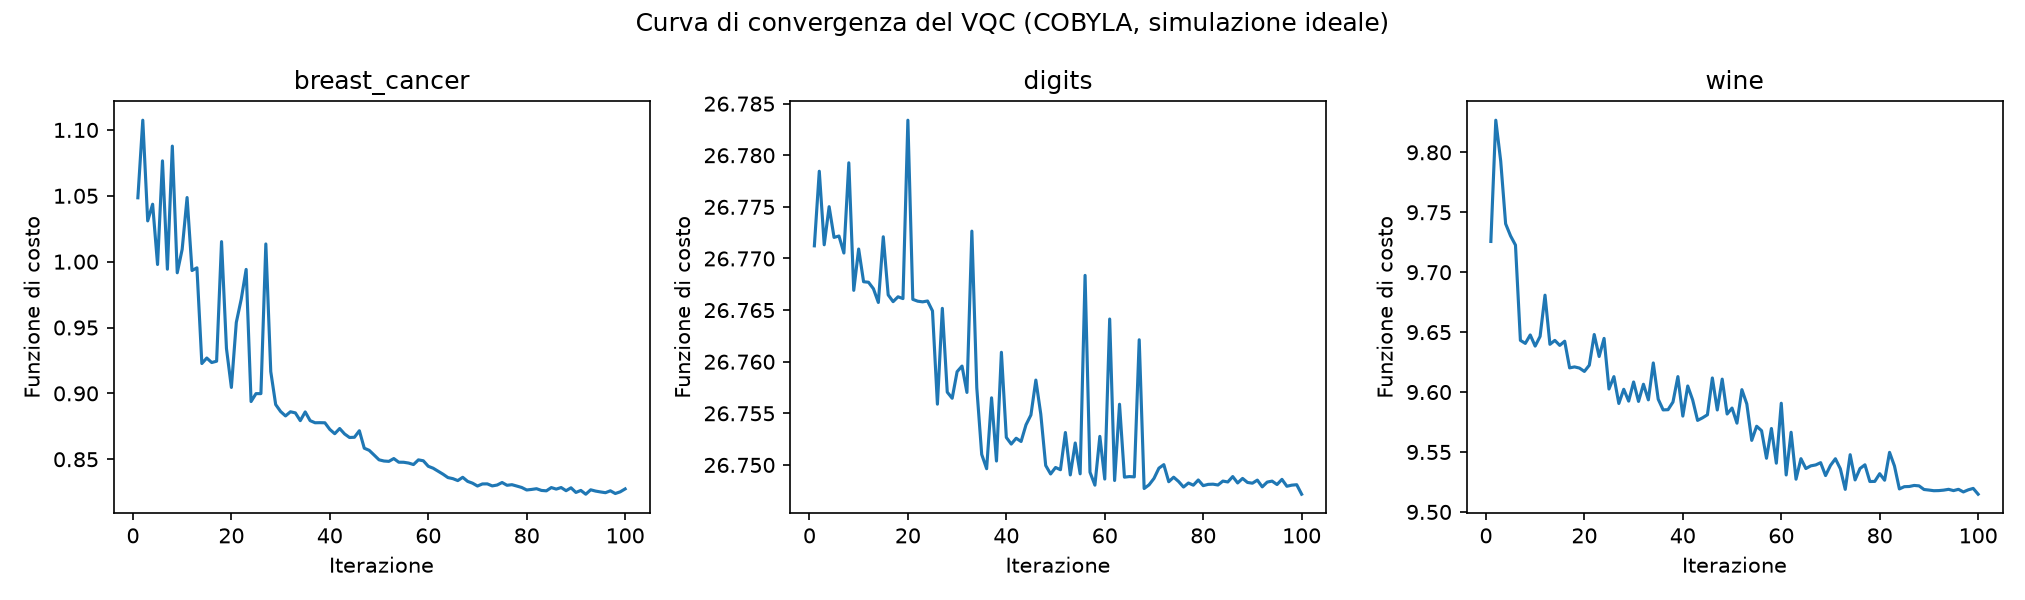
\includegraphics[width=\textwidth]{experiments/results/figures/vqc_convergenza.png}
    \caption{Curva di convergenza della funzione di costo durante l'addestramento del VQC, un pannello per dataset con scala dell'asse y indipendente (i valori assoluti della funzione di costo non sono confrontabili tra dataset).}
    \label{fig:convergenza_vqc}
\end{figure}

\section{Risultati: Breast Cancer Wisconsin}
\label{sec:risultati_breast_cancer}

\subsection{Simulazione ideale}
La Tabella~\ref{tab:risultati_breast_cancer_ideale} riporta le performance dei modelli classici e quantistici sul dataset Breast Cancer Wisconsin, valutate in condizioni di simulazione ideale priva di rumore (\texttt{StatevectorSampler}, Sezione~\ref{sec:impl_backend}).

\begin{table}[htbp]
\centering
\caption{Risultati sul dataset Breast Cancer Wisconsin, simulazione ideale.}
\label{tab:risultati_breast_cancer_ideale}
{\renewcommand{\arraystretch}{1.5} % aumenta lo spazio verticale tra le righe
\footnotesize
\begin{tabular}{>{\raggedright\arraybackslash}p{2.2cm}ccccc}
\toprule
\textbf{Modello} & \textbf{Accuratezza} & \thead{\textbf{Precisione}\\\textbf{(macro)}} & \thead{\textbf{Richiamo}\\\textbf{(macro)}} & \thead{\textbf{F1-score}\\\textbf{(macro)}} & \thead{\textbf{Tempo}\\\textbf{(s)}} \\
\midrule
Logistic Regression & 0,965 & 0,962 & 0,962 & 0,962 & 0,001 \\
SVM (RBF) & 0,956 & 0,955 & 0,950 & 0,953 & 0,001 \\
Random Forest & 0,930 & 0,925 & 0,925 & 0,925 & 0,025 \\
QSVC & 0,746 & 0,727 & 0,714 & 0,719 & 279,22 \\
VQC & 0,728 & 0,732 & 0,661 & 0,666 & 83,72 \\
\bottomrule
\end{tabular}
}
\end{table}

\begin{figure}[htbp]
    \centering
    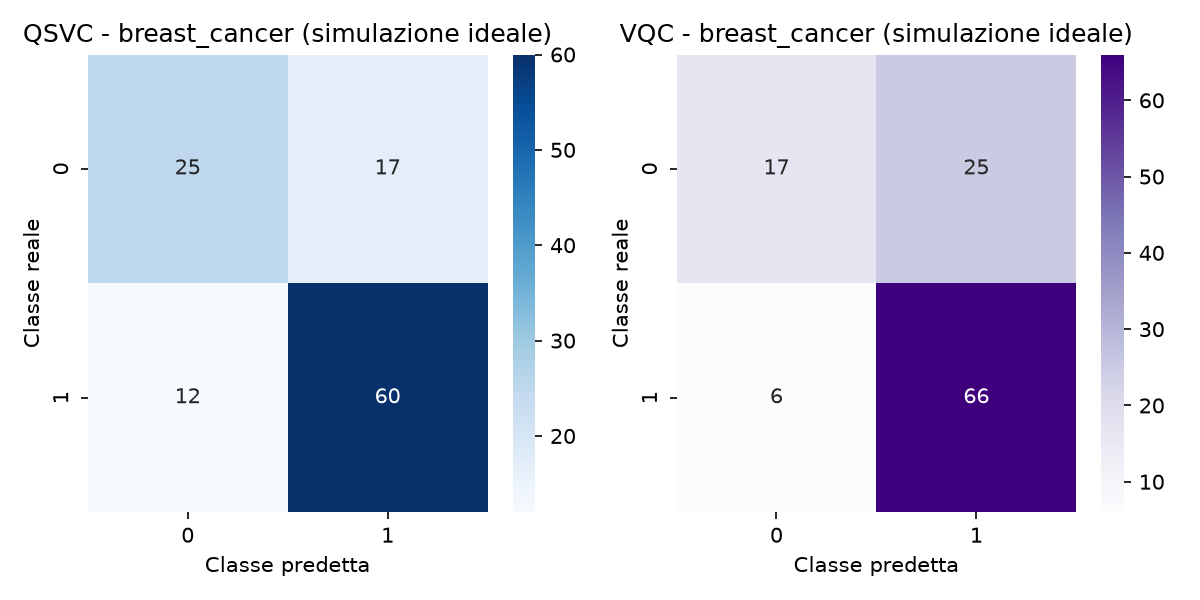
\includegraphics[width=0.85\textwidth]{experiments/results/figures/confusion_matrix_breast_cancer_ideale.png}
    \caption{Matrici di confusione dei modelli quantistici sul dataset Breast Cancer Wisconsin (simulazione ideale).}
    \label{fig:confusion_breast_cancer_ideale}
\end{figure}

\subsection{Simulazione con modello di rumore}
La Tabella~\ref{tab:risultati_breast_cancer_rumore} riporta le medesime metriche ottenute utilizzando il simulatore Qiskit Aer con modello di rumore calibrato su un backend reale (Sezione~\ref{sec:impl_backend}), permettendo di quantificare il degrado di performance atteso rispetto alla simulazione ideale.
\newline
\begin{table}[htbp]
\centering
\caption{Risultati sul dataset Breast Cancer Wisconsin, simulazione con modello di rumore.}
\label{tab:risultati_breast_cancer_rumore}
{\renewcommand{\arraystretch}{1.5} % aumenta lo spazio verticale tra le righe
\footnotesize
\begin{tabular}{>{\raggedright\arraybackslash}p{2.2cm}ccccc}
\toprule
\textbf{Modello} & \textbf{Accuratezza} & \thead{\textbf{Precisione}\\\textbf{(macro)}} & \thead{\textbf{Richiamo}\\\textbf{(macro)}} & \thead{\textbf{F1-score}\\\textbf{(macro)}} & \thead{\textbf{Tempo}\\\textbf{(s)}} \\
\midrule
QSVC & 0,600 & 0,316 & 0,462 & 0,375 & 28,38 \\
VQC & 0,300 & 0,330 & 0,330 & 0,300 & 122,10 \\
\bottomrule
\end{tabular}
}
\end{table}

\subsection{Hardware quantistico reale}
L'esecuzione su hardware quantistico reale non è stata completata per questo dataset (né per gli altri due), per i motivi documentati nella Sezione~\ref{sec:limiti_studio}: il piano gratuito di IBM Quantum Platform (10 minuti di QPU per finestra di 28 giorni) si è esaurito dopo un numero di job insufficiente a completare anche un solo modello, e il passaggio a un piano a consumo avrebbe comportato un costo non sostenibile entro la scadenza di consegna di questo lavoro. La Tabella~\ref{tab:risultati_breast_cancer_hardware}, mantenuta a scopo di documentazione della struttura sperimentale prevista, riporta questa limitazione al posto dei valori numerici.

\begin{table}[htbp]
\centering
\caption{Risultati sul dataset Breast Cancer Wisconsin, esecuzione su hardware quantistico reale (\textbf{non completata}).}
\label{tab:risultati_breast_cancer_hardware}
{\renewcommand{\arraystretch}{1.5} % aumenta lo spazio verticale tra le righe
\footnotesize
\begin{tabular}{>{\raggedright\arraybackslash}p{2.2cm}cccc>{\raggedright\arraybackslash}p{2cm}}
\toprule
\textbf{Modello} & \textbf{Backend} & \textbf{Accuratezza} & \thead{\textbf{F1-score}\\\textbf{(macro)}} & \thead{\textbf{Tempo}\\\textbf{(s)}} & \thead{\textbf{Profondità}\\\textbf{circuito}} \\
\midrule
QSVC & --- & \multicolumn{4}{c}{Non completato (Sezione~\ref{sec:limiti_studio})} \\
VQC & --- & \multicolumn{4}{c}{Non completato (Sezione~\ref{sec:limiti_studio})} \\
\bottomrule
\end{tabular}
}
\end{table}

\section{Risultati: Wine}
\label{sec:risultati_wine}

\subsection{Simulazione ideale}
La Tabella~\ref{tab:risultati_wine_ideale} riporta i risultati ottenuti sul dataset Wine, problema di classificazione multiclasse a tre categorie, in condizioni di simulazione ideale.

\begin{table}[htbp]
\centering
\caption{Risultati sul dataset Wine, simulazione ideale.}
\label{tab:risultati_wine_ideale}
{\renewcommand{\arraystretch}{1.5} % aumenta lo spazio verticale tra le righe
\footnotesize
\begin{tabular}{>{\raggedright\arraybackslash}p{2.2cm}ccccc}
\toprule
\textbf{Modello} & \textbf{Accuratezza} & \thead{\textbf{Precisione}\\\textbf{(macro)}} & \thead{\textbf{Richiamo}\\\textbf{(macro)}} & \thead{\textbf{F1-score}\\\textbf{(macro)}} & \thead{\textbf{Tempo}\\\textbf{(s)}} \\
\midrule
Logistic Regression & 1,000 & 1,000 & 1,000 & 1,000 & 0,002 \\
SVM (RBF) & 0,944 & 0,951 & 0,943 & 0,945 & 0,001 \\
Random Forest & 1,000 & 1,000 & 1,000 & 1,000 & 0,042 \\
QSVC & 0,750 & 0,818 & 0,726 & 0,742 & 31,40 \\
VQC & 0,389 & 0,260 & 0,357 & 0,301 & 30,44 \\
\bottomrule
\end{tabular}
}
\end{table}

\subsection{Simulazione con modello di rumore e hardware reale}
Analogamente a quanto riportato per il dataset Breast Cancer Wisconsin, la Tabella~\ref{tab:risultati_wine_rumore_hw} riassume i risultati ottenuti sul dataset Wine in simulazione con rumore; l'esecuzione su hardware reale non è stata completata, per i motivi documentati nella Sezione~\ref{sec:limiti_studio}.

\begin{table}[htbp]
\centering
\caption{Risultati sul dataset Wine: simulazione con rumore (\textbf{hardware reale non completato}).}
\label{tab:risultati_wine_rumore_hw}
{\renewcommand{\arraystretch}{1.5} % aumenta lo spazio verticale tra le righe
\footnotesize
\begin{tabular}{>{\raggedright\arraybackslash}p{1.6cm}>{\raggedright\arraybackslash}p{3cm}ccc}
\toprule
\textbf{Modello} & \textbf{Ambiente} & \textbf{Accuratezza} & \thead{\textbf{F1-score}\\\textbf{(macro)}} & \thead{\textbf{Tempo}\\\textbf{(s)}} \\
\midrule
QSVC & Simulazione con rumore & 0,650 & 0,571 & 33,36 \\
QSVC & Hardware reale & \multicolumn{3}{c}{Non completato (Sezione~\ref{sec:limiti_studio})} \\
VQC & Simulazione con rumore & 0,250 & 0,189 & 134,18 \\
VQC & Hardware reale & \multicolumn{3}{c}{Non completato (Sezione~\ref{sec:limiti_studio})} \\
\bottomrule
\end{tabular}
}
\end{table}

\begin{figure}[htbp]
    \centering
    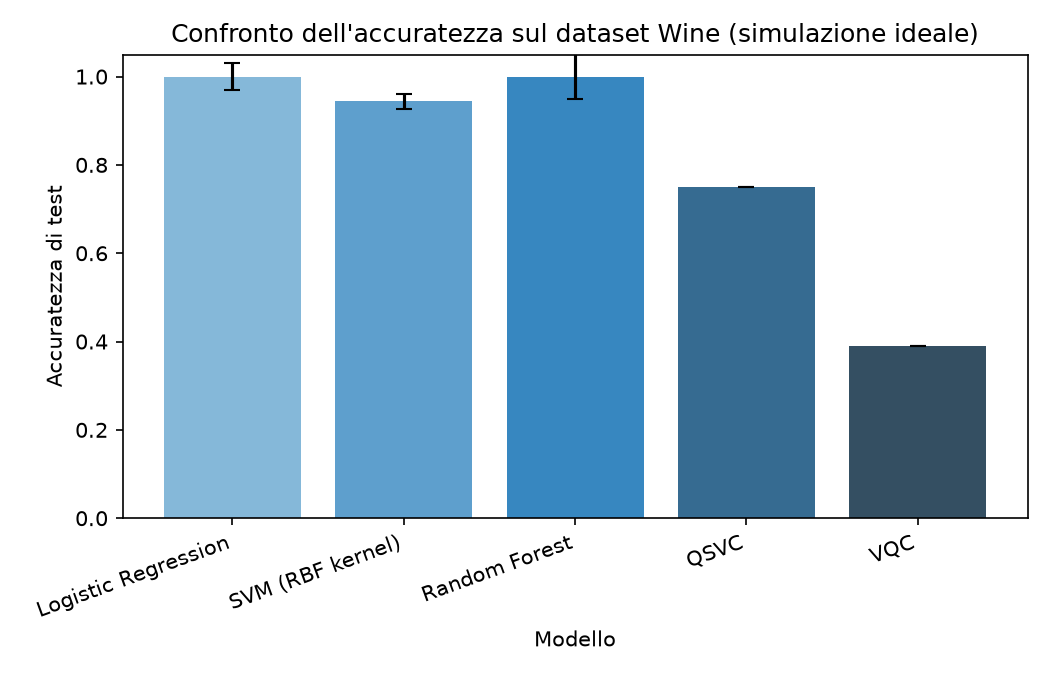
\includegraphics[width=0.85\textwidth]{experiments/results/figures/wine_accuracy_comparison.png}
    \caption{Confronto dell'accuratezza tra modelli classici e quantistici sul dataset Wine.}
    \label{fig:wine_accuracy_comparison}
\end{figure}

\section{Risultati: Digits}
\label{sec:risultati_digits}

\subsection{Simulazione ideale}
Il dataset Digits, caratterizzato dalla dimensionalità originaria più elevata (64 feature, ridotte a 6 componenti principali secondo quanto riportato in Tabella~\ref{tab:pca_componenti}) e da un problema di classificazione multiclasse a dieci categorie, rappresenta il caso più impegnativo tra quelli considerati. La Tabella~\ref{tab:risultati_digits_ideale} riporta i risultati ottenuti in simulazione ideale.

\begin{table}[htbp]
\centering
\caption{Risultati sul dataset Digits, simulazione ideale.}
\label{tab:risultati_digits_ideale}
{\renewcommand{\arraystretch}{1.5} % aumenta lo spazio verticale tra le righe
\footnotesize
\begin{tabular}{>{\raggedright\arraybackslash}p{2.2cm}ccccc}
\toprule
\textbf{Modello} & \textbf{Accuratezza} & \thead{\textbf{Precisione}\\\textbf{(macro)}} & \thead{\textbf{Richiamo}\\\textbf{(macro)}} & \thead{\textbf{F1-score}\\\textbf{(macro)}} & \thead{\textbf{Tempo}\\\textbf{(s)}} \\
\midrule
Logistic Regression & 0,844 & 0,846 & 0,844 & 0,841 & 0,007 \\
SVM (RBF) & 0,958 & 0,960 & 0,958 & 0,958 & 0,010 \\
Random Forest & 0,919 & 0,921 & 0,919 & 0,919 & 0,265 \\
QSVC & 0,286 & 0,287 & 0,286 & 0,286 & 3803,29 \\
VQC & 0,097 & 0,019 & 0,097 & 0,032 & 356,35 \\
\bottomrule
\end{tabular}
}
\end{table}

\subsection{Effetto della riduzione dimensionale}
Data l'elevata dimensionalità originaria del dataset Digits, è stata condotta un'analisi di sensitività empirica delle performance dei modelli al variare del numero di componenti principali utilizzate, anticipata nella Sezione~\ref{sec:pca} come verifica empirica della scelta del numero di componenti. I risultati di tale analisi sono riportati in Tabella~\ref{tab:digits_sensitivity_pca}.

\begin{table}[htbp]
\centering
\caption{Accuratezza del modello QSVC sul dataset Digits al variare del numero di componenti principali (e quindi di qubit) utilizzate.}
\label{tab:digits_sensitivity_pca}
\begin{tabular}{cccc}
\toprule
\textbf{Componenti PCA} & \textbf{Qubit} & \textbf{Varianza spiegata} & \textbf{Accuratezza QSVC} \\
\midrule
4 & 4 & 0,486 & 0,328 \\
5 & 5 & 0,542 & 0,278 \\
6 & 6 & 0,591 & 0,286 \\
8 & 8 & 0,669 & 0,258 \\
\bottomrule
\end{tabular}
\end{table}

\subsection{Simulazione con rumore e hardware reale}
La Tabella~\ref{tab:risultati_digits_rumore_hw} riporta i risultati ottenuti sul dataset Digits in simulazione con rumore; l'esecuzione su hardware reale non è stata completata, per i motivi documentati nella Sezione~\ref{sec:limiti_studio}.

\begin{table}[htbp]
\centering
\caption{Risultati sul dataset Digits: simulazione con rumore (\textbf{hardware reale non completato}).}
\label{tab:risultati_digits_rumore_hw}
{\renewcommand{\arraystretch}{1.5} % aumenta lo spazio verticale tra le righe
\footnotesize
\begin{tabular}{>{\raggedright\arraybackslash}p{1.6cm}>{\raggedright\arraybackslash}p{3cm}ccc}
\toprule
\textbf{Modello} & \textbf{Ambiente} & \textbf{Accuratezza} & \thead{\textbf{F1-score}\\\textbf{(macro)}} & \thead{\textbf{Tempo}\\\textbf{(s)}} \\
\midrule
QSVC & Simulazione con rumore & 0,100 & 0,075 & 42,44 \\
QSVC & Hardware reale & \multicolumn{3}{c}{Non completato (Sezione~\ref{sec:limiti_studio})} \\
VQC & Simulazione con rumore & 0,100 & 0,033 & 163,59 \\
VQC & Hardware reale & \multicolumn{3}{c}{Non completato (Sezione~\ref{sec:limiti_studio})} \\
\bottomrule
\end{tabular}
}
\end{table}

\section{Analisi comparativa trasversale}
\label{sec:analisi_comparativa}

\subsection{Confronto dell'accuratezza tra dataset e modelli}
\label{sec:confronto_accuratezza}

La Tabella~\ref{tab:confronto_globale_accuratezza} riassume l'accuratezza di test ottenuta da ciascun modello sui tre dataset, in condizioni di simulazione ideale, permettendo un confronto diretto e sintetico tra gli approcci classici e quantistici oggetto di questo lavoro.

\begin{table}[htbp]
\centering
\caption{Confronto globale dell'accuratezza di test tra tutti i modelli e tutti i dataset (simulazione ideale).}
\label{tab:confronto_globale_accuratezza}
\begin{tabular}{lccc}
\toprule
\textbf{Modello} & \textbf{Breast Cancer Wisconsin} & \textbf{Wine} & \textbf{Digits} \\
\midrule
Logistic Regression & 0,965 & 1,000 & 0,844 \\
SVM (RBF) & 0,956 & 0,944 & 0,958 \\
Random Forest & 0,930 & 1,000 & 0,919 \\
QSVC & 0,746 & 0,750 & 0,286 \\
VQC & 0,728 & 0,389 & 0,097 \\
\bottomrule
\end{tabular}
\end{table}

\begin{figure}[htbp]
    \centering
    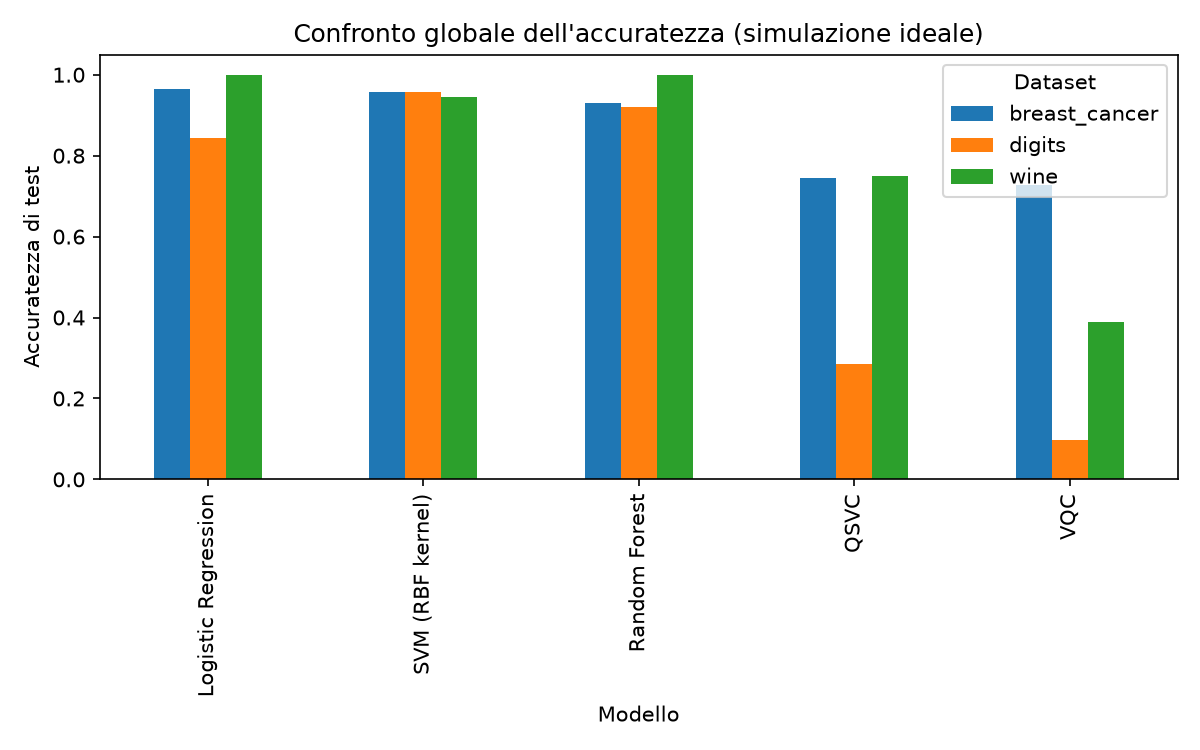
\includegraphics[width=0.85\textwidth]{experiments/results/figures/confronto_globale_accuratezza.png}
    \caption{Confronto globale dell'accuratezza tra modelli classici e quantistici sui tre dataset.}
    \label{fig:confronto_globale_accuratezza}
\end{figure}

\subsection{Costo computazionale e tempi di esecuzione}
\label{sec:costo_computazionale}

Oltre alla qualità predittiva, il protocollo sperimentale descritto nella Sezione~\ref{sec:protocollo_sperimentale} prevede la raccolta dei tempi di esecuzione e, per i modelli quantistici, del numero di circuiti eseguiti e della relativa profondità. La Tabella~\ref{tab:costo_computazionale} riassume queste grandezze, permettendo di discutere il costo computazionale relativo degli approcci classici e quantistici a parità di dataset.

\begin{table}[htbp]
\centering
\caption{Costo computazionale comparato tra modelli classici e quantistici (simulazione ideale, dataset Breast Cancer Wisconsin).}
\label{tab:costo_computazionale}
{\renewcommand{\arraystretch}{1.5} % aumenta lo spazio verticale tra le righe
\footnotesize
\begin{tabular}{>{\raggedright\arraybackslash}p{2.2cm}ccc}
\toprule
\textbf{Modello} & \thead{\textbf{Tempo di}\\\textbf{addestramento (s)}} & \thead{\textbf{N. circuiti}\\\textbf{eseguiti}} & \thead{\textbf{Profondità}\\\textbf{del circuito}} \\
\midrule
Logistic Regression & 0,001 & --- & --- \\
SVM (RBF) & 0,001 & --- & --- \\
Random Forest & 0,025 & --- & --- \\
QSVC & 279,22 & 155.155 & 19 \\
VQC & 83,72 & 45.614 & 29 \\
\bottomrule
\end{tabular}
}

\medskip
{\footnotesize Il tempo di addestramento riportato per i modelli classici è il tempo del solo fit finale, agli iperparametri selezionati dalla ricerca a griglia (Sezione~\ref{sec:impl_classici}), misurato in modo omogeneo al fit singolo di QSVC e VQC; il costo della ricerca a griglia stessa (\texttt{grid\_search\_time\_s}, Sezione~\ref{sec:impl_orchestrazione}) non è incluso in questa colonna.}
\end{table}

Come atteso sulla base della discussione teorica svolta nella Sezione~\ref{sec:complessita_qml} del Capitolo~\ref{cap:quantum_machine_learning}, i modelli quantistici, in particolare in fase di simulazione, presentano tempi di addestramento superiori rispetto ai modelli classici corrispondenti, a causa dell'overhead introdotto dalla simulazione dello stato quantistico e, nel caso del QSVC, dal calcolo della matrice di kernel completa tra tutte le coppie di campioni di addestramento; il confronto è omogeneo poiché, come descritto nella Sezione~\ref{sec:impl_orchestrazione}, per tutti i modelli il tempo misurato è quello del solo fit finale a iperparametri fissati, escludendo per i modelli classici il costo della ricerca a griglia.

\subsection{Effetto del rumore e del passaggio a hardware reale}
\label{sec:effetto_rumore}

La Figura~\ref{fig:degrado_performance} illustra il degrado di performance osservato passando dalla simulazione ideale alla simulazione con modello di rumore, per i modelli QSVC e VQC sui tre dataset considerati; il terzo ambiente previsto dalla strategia progressiva di valutazione, l'esecuzione su hardware quantistico reale, non compare in figura poiché non è stato possibile completarla, per i motivi documentati nella Sezione~\ref{sec:limiti_studio}.

\begin{figure}[htbp]
    \centering
    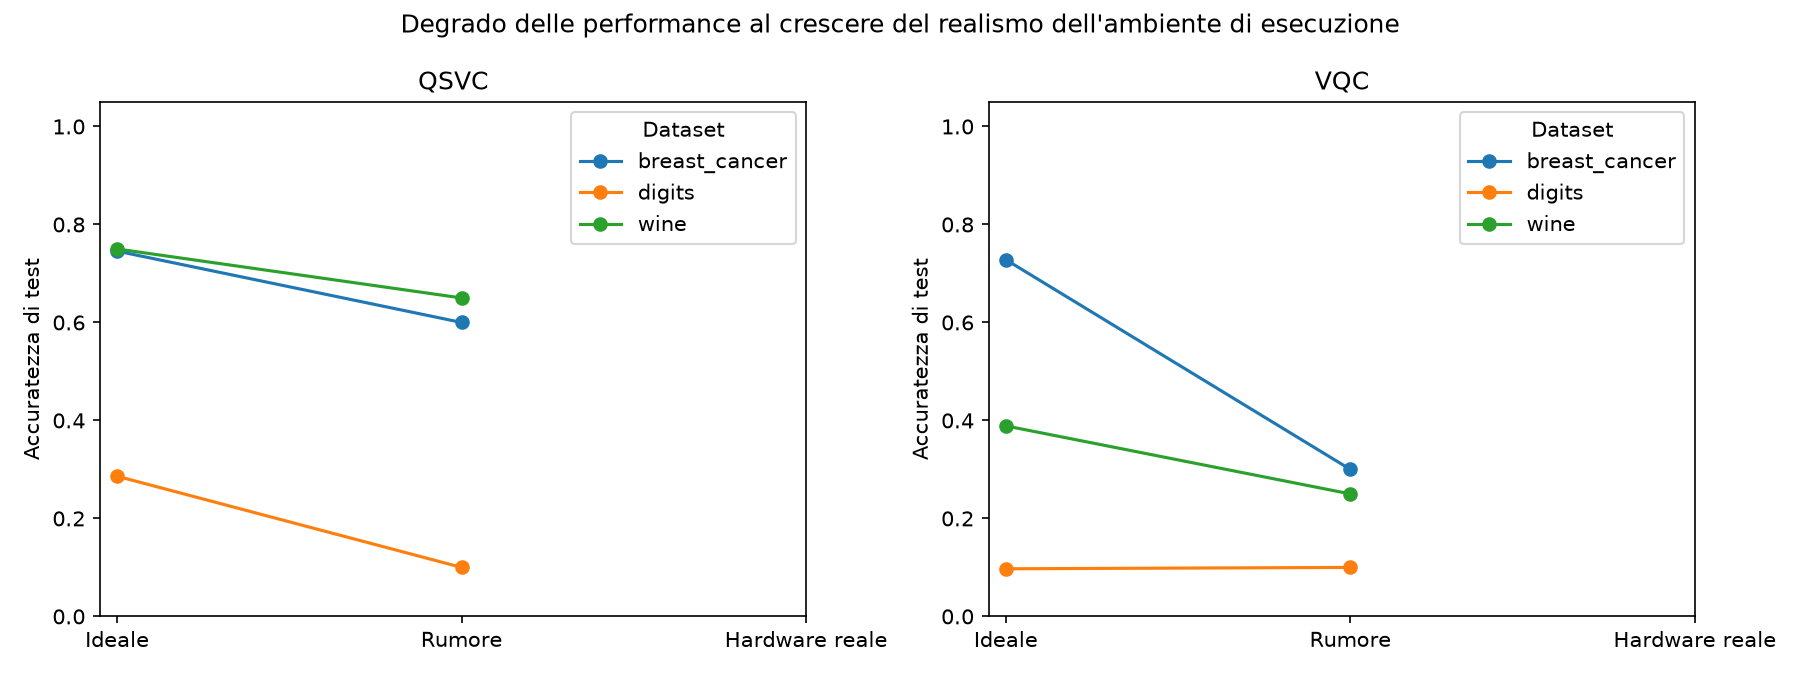
\includegraphics[width=0.85\textwidth]{experiments/results/figures/degrado_performance_ambienti.png}
    \caption{Degrado delle performance dei modelli quantistici tra simulazione ideale e simulazione con modello di rumore (l'ambiente hardware reale non è presente, si veda il testo).}
    \label{fig:degrado_performance}
\end{figure}

\subsection{Confronto tra ottimizzatori per il VQC}
\label{sec:confronto_ottimizzatori}

Come anticipato nella Sezione~\ref{sec:impl_vqc}, è stato condotto un confronto preliminare tra gli ottimizzatori COBYLA e SPSA per l'addestramento del VQC, i cui risultati sono riportati in Tabella~\ref{tab:confronto_ottimizzatori}. Per un confronto equo dell'inizializzazione, il seed di \texttt{algorithm\_globals.random} (Sezione~\ref{sec:impl_orchestrazione}) è fissato immediatamente prima di ciascuna delle due costruzioni del VQC, in modo che entrambi gli ottimizzatori partano dallo stesso punto iniziale casuale dei parametri variazionali; senza questo accorgimento, differenze nell'accuratezza o nella velocità di convergenza tra COBYLA e SPSA potrebbero essere dovute a un'inizializzazione diversa anziché all'ottimizzatore in sé.

Fissare l'inizializzazione non basta però a rendere equo il \emph{budget} di valutazione della funzione di costo tra i due ottimizzatori, poiché in qiskit-machine-learning il parametro \texttt{maxiter} ha semantica diversa nei due casi: per \texttt{COBYLA} indica il numero massimo di valutazioni della funzione di costo, mentre per \texttt{SPSA} indica il numero di iterazioni, ciascuna delle quali richiede almeno due valutazioni (oltre a un'eventuale fase di calibrazione iniziale). Impostando \newline\texttt{maxiter=VQC\_MAXITER} per entrambi, SPSA dispone quindi tipicamente di un budget di valutazioni più ampio di COBYLA, nonostante il valore nominale di \texttt{maxiter} sia identico; di conseguenza la colonna "Iterazioni per la convergenza" (\texttt{n\_iterations}, lunghezza della cronologia della funzione di costo raccolta dalla rispettiva callback) conta unità non direttamente confrontabili tra i due ottimizzatori. Per questo motivo il sampler è wrappato in un \texttt{CountingSampler} (Sezione~\ref{sec:impl_backend}) anche in questo confronto, e la Tabella~\ref{tab:confronto_ottimizzatori} riporta anche \texttt{n\_circuits}, il numero di circuiti quantistici effettivamente eseguiti durante l'addestramento: è quest'ultima colonna, e non "Iterazioni per la convergenza", a fornire una base di confronto realmente omogenea del costo computazionale tra i due ottimizzatori.

\begin{table}[htbp]
\centering
\caption{Confronto tra gli ottimizzatori COBYLA e SPSA per l'addestramento del VQC (dataset Breast Cancer Wisconsin, simulazione ideale).}
\label{tab:confronto_ottimizzatori}
{\renewcommand{\arraystretch}{1.5} % aumenta lo spazio verticale tra le righe
\footnotesize
\begin{tabular}{>{\raggedright\arraybackslash}p{2.2cm}cccc}
\toprule
\textbf{Ottimizzatore} & \thead{\textbf{Accuratezza}\\\textbf{di test}} & \thead{\textbf{Iterazioni per}\\\textbf{la convergenza}} & \thead{\textbf{N. circuiti}\\\textbf{eseguiti}} & \thead{\textbf{Tempo}\\\textbf{totale (s)}} \\
\midrule
COBYLA & 0,728 & 100 & 45.614 & 84,91 \\
SPSA & 0,693 & 100 & 159.364 & 295,26 \\
\bottomrule
\end{tabular}
}

\medskip
{\footnotesize La colonna "Iterazioni per la convergenza" conta le invocazioni della rispettiva callback e non è direttamente confrontabile tra i due ottimizzatori (si veda il testo); "N. circuiti eseguiti" è la base di confronto del costo computazionale omogenea tra COBYLA e SPSA.}
\end{table}

\section{Discussione dei risultati}
\label{sec:discussione_risultati}

\subsection{Confronto tra modelli classici e quantistici}
Sulla base dei risultati riportati nelle Sezioni~\ref{sec:risultati_breast_cancer}--\ref{sec:risultati_digits} e riassunti in Tabella~\ref{tab:confronto_globale_accuratezza}, nelle configurazioni quantistiche adottate (Tabella~\ref{tab:configurazione_completa}) i modelli classici di baseline ottengono prestazioni superiori a quelle di entrambi i modelli quantistici su tutti e tre i dataset, senza eccezioni. Su Breast Cancer Wisconsin il divario è relativamente contenuto (Logistic Regression 0,965 contro 0,746 del QSVC e 0,728 del VQC, una differenza di circa 22 punti percentuali con il modello quantistico migliore); su Wine il divario si allarga (Random Forest e Logistic Regression raggiungono l'accuratezza massima, 1,000, contro 0,750 del QSVC); su Digits, il dataset con la dimensionalità originaria più elevata e l'unico multiclasse a dieci categorie, il divario diventa marcato, con SVM a 0,958 contro appena 0,286 del QSVC e 0,097 del VQC, quest'ultimo sostanzialmente equivalente alla classificazione casuale (1/10 per un problema a dieci classi bilanciate). Nelle configurazioni testate i modelli quantistici non eguagliano mai le baseline classiche e il divario tende ad ampliarsi al crescere della complessità del problema (numero di classi, dimensionalità originaria), un andamento opposto a quanto ci si aspetterebbe se fosse presente un vantaggio quantistico legato alla capacità di rappresentare correlazioni complesse. Questo risultato è coerente con la discussione teorica sui possibili vantaggi del machine learning quantistico svolta nella Sezione~\ref{sec:data_encoding} del Capitolo~\ref{cap:quantum_machine_learning}, secondo cui un eventuale vantaggio quantistico, ove presente, è atteso principalmente su dataset con strutture di correlazione difficili da rappresentare efficientemente con kernel classici: condizione che, con ogni probabilità, i tre dataset reali e relativamente semplici utilizzati in questo lavoro non soddisfano. L'elevata accuratezza raggiunta dalla SVM con kernel RBF (0,956, 0,944 e 0,958 sui tre dataset) suggerisce che un kernel classico sia già sufficiente a catturarne la struttura rilevante, ma questa ipotesi non è stata verificata direttamente, ad esempio analizzando la struttura di correlazione delle feature.

Questi risultati vanno inoltre letti come riferiti alle configurazioni di QSVC e VQC adottate in questo lavoro, per i motivi discussi nella Sezione~\ref{sec:limiti_studio}.

\subsection{QSVC vs VQC}
Il confronto diretto tra i due modelli quantistici implementati permette di discutere le differenze pratiche tra l'approccio a kernel quantistico (QSVC) e l'approccio variazionale (VQC), introdotte a livello teorico nella Sezione~\ref{sec:confronto_qsvc_vqc} del Capitolo~\ref{cap:quantum_machine_learning}. In simulazione ideale il QSVC eguaglia o supera il VQC su tutti e tre i dataset (Tabella~\ref{tab:confronto_globale_accuratezza}): il divario è modesto su Breast Cancer Wisconsin (0,746 contro 0,728) ma sostanziale su Wine (0,750 contro 0,389) e su Digits (0,286 contro 0,097, dove il VQC si attesta al livello della classificazione casuale). Questo risultato è coerente con l'assenza, nell'approccio a kernel, del problema dei barren plateaus discusso nella Sezione~\ref{sec:barren_plateaus} del Capitolo~\ref{cap:quantum_machine_learning}: la funzione obiettivo del QSVC (la massimizzazione del margine dell'SVM sul kernel calcolato) è convessa e non richiede un'ottimizzazione iterativa dei parametri del circuito, mentre il VQC deve navigare un \textit{landscape} non convesso che può presentare gradienti prossimi a zero, specialmente all'aumentare del numero di qubit e della profondità del circuito (rispettivamente 6 e 35 per Digits, i valori più elevati tra i tre dataset, si veda la Tabella~\ref{tab:risultati_digits_ideale}). L'indizio più diretto di questa difficoltà è la curva di convergenza del VQC su Digits (Figura~\ref{fig:convergenza_vqc}): la funzione di costo scende da 26,77 a 26,75 in 100 iterazioni di COBYLA, una variazione relativa (circa lo 0,1\%) di due ordini di grandezza inferiore a quella osservata su Breast Cancer Wisconsin (circa il 22\%) e su Wine (circa il 3\%) a parità di iterazioni, un comportamento compatibile con un ottimizzatore che si muove in una regione a gradiente prossimo allo zero del \textit{landscape}, piuttosto che con una discesa efficace verso un minimo. Va però precisato che i \textit{barren plateaus} non sono stati misurati direttamente in questo lavoro (ad esempio stimando la varianza dei gradienti al variare del numero di qubit): l'andamento osservato è coerente con questa interpretazione, ma potrebbe dipendere anche da altri fattori, come il numero limitato di iterazioni di COBYLA, la scelta dell'ansatz o l'inizializzazione dei parametri, e non va quindi considerato una prova della presenza del fenomeno.

Il confronto tra gli ottimizzatori COBYLA e SPSA per il VQC (Tabella~\ref{tab:confronto_ottimizzatori}, dataset Breast Cancer Wisconsin) mostra COBYLA leggermente più accurato (0,728 contro 0,693 di SPSA) pur utilizzando meno di un terzo dei circuiti quantistici effettivamente eseguiti (45.614 contro 159.364) a parità di \texttt{maxiter} nominale, coerente con quanto discusso in Sezione~\ref{sec:impl_vqc} circa la maggiore economia di valutazioni di COBYLA rispetto a SPSA per problemi di questa scala, sebbene quest'ultimo sia teoricamente più robusto in presenza di rumore nella valutazione della funzione di costo.

\subsection{Effetto della dimensionalità e della riduzione tramite PCA}
I risultati riportati nella Sezione~\ref{sec:risultati_digits}, in particolare l'analisi di sensitività riportata in Tabella~\ref{tab:digits_sensitivity_pca}, permettono di discutere l'impatto della riduzione dimensionale sulle performance dei modelli quantistici. Il dato più significativo è che l'accuratezza del QSVC \emph{non} migliora in modo sistematico all'aumentare del numero di componenti principali (e quindi di qubit) utilizzate: il massimo si osserva alla configurazione più piccola testata (4 componenti, accuratezza 0,328), seguito da un calo a 5 componenti (0,278), un lieve recupero a 6 (0,286, la configurazione principale usata nel resto del capitolo) e un ulteriore calo a 8 componenti (0,258, il valore più basso dell'intera analisi), nonostante la varianza spiegata cumulata cresca in modo monotono da 0,486 a 0,669 nello stesso intervallo (Tabella~\ref{tab:digits_sensitivity_pca}). In altre parole, un sottospazio a più alta dimensionalità (e quindi, in linea di principio, più informativo rispetto ai dati originari) non si traduce in un kernel quantistico più efficace per la classificazione: un andamento opposto a quello tipicamente atteso per i modelli classici, dove più varianza spiegata trattenuta dalla PCA tende a correlare con migliori prestazioni a valle. Questo andamento è compatibile con i fenomeni di concentrazione del kernel discussi in letteratura per i kernel quantistici basati su feature map di tipo \texttt{ZZFeatureMap}\footnote{Thanasilp, S., Wang, S., Cerezo, M., \& Holmes, Z. (2024). Exponential concentration in quantum kernel methods. \textit{Nature Communications}, 15, Articolo 5200. \url{https://doi.org/10.1038/s41467-024-49287-w}.}, per cui l'aumento del numero di qubit può ridurre la capacità discriminante del kernel calcolato anziché aumentarla. Si tratta però di un'interpretazione plausibile e non di una causa dimostrata: la concentrazione del kernel non è stata misurata direttamente (ad esempio tramite la varianza degli elementi della matrice di kernel al crescere dei qubit), l'analisi di sensitività si basa su una singola suddivisione train/test e su un solo seed, e differenze anche di pochi punti percentuali possono rientrare nella normale variabilità campionaria; non è inoltre escluso il contributo di altri fattori, come la scelta della feature map o la perdita di informazione dovuta alla PCA. Il vincolo pratico sul numero di qubit discusso nella Sezione~\ref{sec:pca}, motivato da ragioni di trattabilità computazionale, risulta quindi, alla luce di queste osservazioni, meno penalizzante di quanto inizialmente ipotizzato: la configurazione a 6 componenti scelta per il resto del capitolo non è distante dal massimo osservato nell'intervallo testato, e comunque non è la configurazione con le prestazioni peggiori.

\subsection{Impatto del rumore hardware}
Il confronto tra simulazione ideale e simulazione con modello di rumore, riportato nella Sezione~\ref{sec:effetto_rumore}, consente di quantificare concretamente l'impatto delle limitazioni dell'era NISQ discusse nella Sezione~\ref{sec:rumore_nisq} del Capitolo~\ref{cap:quantum_machine_learning}, limitatamente a questo confronto, poiché il terzo ambiente previsto, l'esecuzione su hardware quantistico reale, non è stato completato (Sezione~\ref{sec:limiti_studio}).

Il degrado è sistematico su entrambi i modelli e su tutti e tre i dataset (Figura~\ref{fig:degrado_performance}), ma sensibilmente più marcato per il VQC che per il QSVC in termini relativi: su Breast Cancer Wisconsin l'accuratezza del QSVC scende dal 0,746 ideale al 0,600 con rumore (-14,6 punti percentuali), mentre quella del VQC scende dal 0,728 al 0,300 (-42,8 punti); su Wine il QSVC passa da 0,750 a 0,650 (-10,0 punti) contro il VQC da 0,389 a 0,250 (-13,9 punti). Su Digits il confronto è meno informativo poiché il VQC è già al livello della classificazione casuale in simulazione ideale (0,097) e resta sostanzialmente invariato con rumore (0,100); il QSVC, che in simulazione ideale manteneva un margine sopra il caso (0,286), collassa anch'esso al livello casuale con rumore (0,100), un degrado di -18,6 punti.

Questa asimmetria tra QSVC e VQC è coerente con la profondità relativa dei circuiti coinvolti nei due approcci (Tabella~\ref{tab:risultati_breast_cancer_ideale} e sezioni corrispondenti per Wine e Digits): il circuito del VQC, che compone la feature map con l'ansatz variazionale, ha una profondità sistematicamente maggiore di quello del solo QSVC (29 contro 19 per Breast Cancer Wisconsin, 32 contro 22 per Wine, 35 contro 25 per Digits) e risulta pertanto esposto a un numero maggiore di operazioni rumorose, con conseguente accumulo di errore più marcato per ogni esecuzione del circuito, indipendentemente dal fatto che il VQC richieda anche, a differenza del QSVC, un'ottimizzazione iterativa dei parametri che il rumore può ulteriormente disturbare.

\subsection{Limiti dello studio e minacce alla validità}
\label{sec:limiti_studio}
Indipendentemente dai risultati numerici ottenuti, è opportuno esplicitare alcuni limiti metodologici propri di questo lavoro, che ne circoscrivono la validità e la generalizzabilità delle conclusioni:
\begin{itemize}
    \item \textbf{Dimensione contenuta dei dataset e del numero di qubit}: i vincoli pratici discussi nella Sezione~\ref{sec:dataset_preprocessing} limitano la sperimentazione a dataset di dimensioni relativamente contenute e a un numero ridotto di qubit (4--6), non rappresentativo delle dimensioni alle quali un eventuale vantaggio quantistico asintotico potrebbe manifestarsi.
    \item \textbf{Perdita di informazione dovuta alla PCA}: come discusso nella Sezione~\ref{sec:pca}, la riduzione dimensionale comporta una perdita di informazione che agisce allo stesso modo su tutti i modelli confrontati, ma che potrebbe penalizzare in misura diversa i modelli quantistici rispetto a quelli classici, data la diversa sensibilità alla struttura delle feature in ingresso.
    \item \textbf{Esecuzione su hardware quantistico reale non completata}: a differenza delle modalità \texttt{ideal} e \texttt{noisy\_simulation}, per le quali la campagna sperimentale è stata completata su tutti e tre i dataset, l'esecuzione su hardware quantistico reale (\texttt{real\_hardware}, Sezione~\ref{sec:esecuzione_hardware_reale}) non è stata completata per nessuno dei tre dataset, per un vincolo pratico riscontrato empiricamente e non pienamente anticipabile in fase di progettazione: il piano gratuito ("Open") di IBM Quantum Platform mette a disposizione solo 10 minuti di tempo di QPU per finestra di 28 giorni scorrevole. Nel tentativo di esecuzione condotto per questo lavoro, la quota si è esaurita dopo appena 9 job (sul solo dataset Breast Cancer Wisconsin, con \texttt{QSVC\_MAX\_CIRCUITS\_PER\_JOB} = 100, si veda il pannello \textit{Workloads} di IBM Quantum Platform in Figura~\ref{fig:ibm_workloads_jobs}), con un tempo medio osservato di circa 109 secondi (1 minuto e 49 secondi) per singolo job, un valore ben superiore al tempo di esecuzione quantistica atteso per 100 circuiti, che suggerisce un overhead fisso non trascurabile per singolo job (accodamento, verifica della calibrazione, dispatch del sistema di controllo), in parte indipendente dal numero di circuiti effettivamente contenuti in ciascuna chiamata. Aumentare la dimensione del chunk (\texttt{QSVC\_REAL\_HARDWARE\_MAX\_CIRCUITS\_PER\_JOB}, si veda il punto seguente) per ridurre il numero di job necessari è una mitigazione plausibile, ma non è stato possibile verificarla empiricamente per mancanza di quota residua. Anche nell'ipotesi più favorevole, completare la campagna sperimentale su hardware reale passando al piano a consumo (\textit{pay-as-you-go}, a partire da 96 \$/minuto secondo il listino IBM al momento della stesura di questo lavoro) avrebbe un costo dell'ordine delle centinaia se non delle migliaia di dollari per singolo dataset, non sostenibile nell'ambito di questo lavoro e incompatibile con la scadenza di consegna fissata. Le tabelle dei risultati su hardware reale (Sezioni~\ref{sec:risultati_breast_cancer}--\ref{sec:risultati_digits}) riportano esplicitamente questa limitazione al posto dei valori numerici.

    \clearpage
    \begin{figure}[htbp]
        \centering
        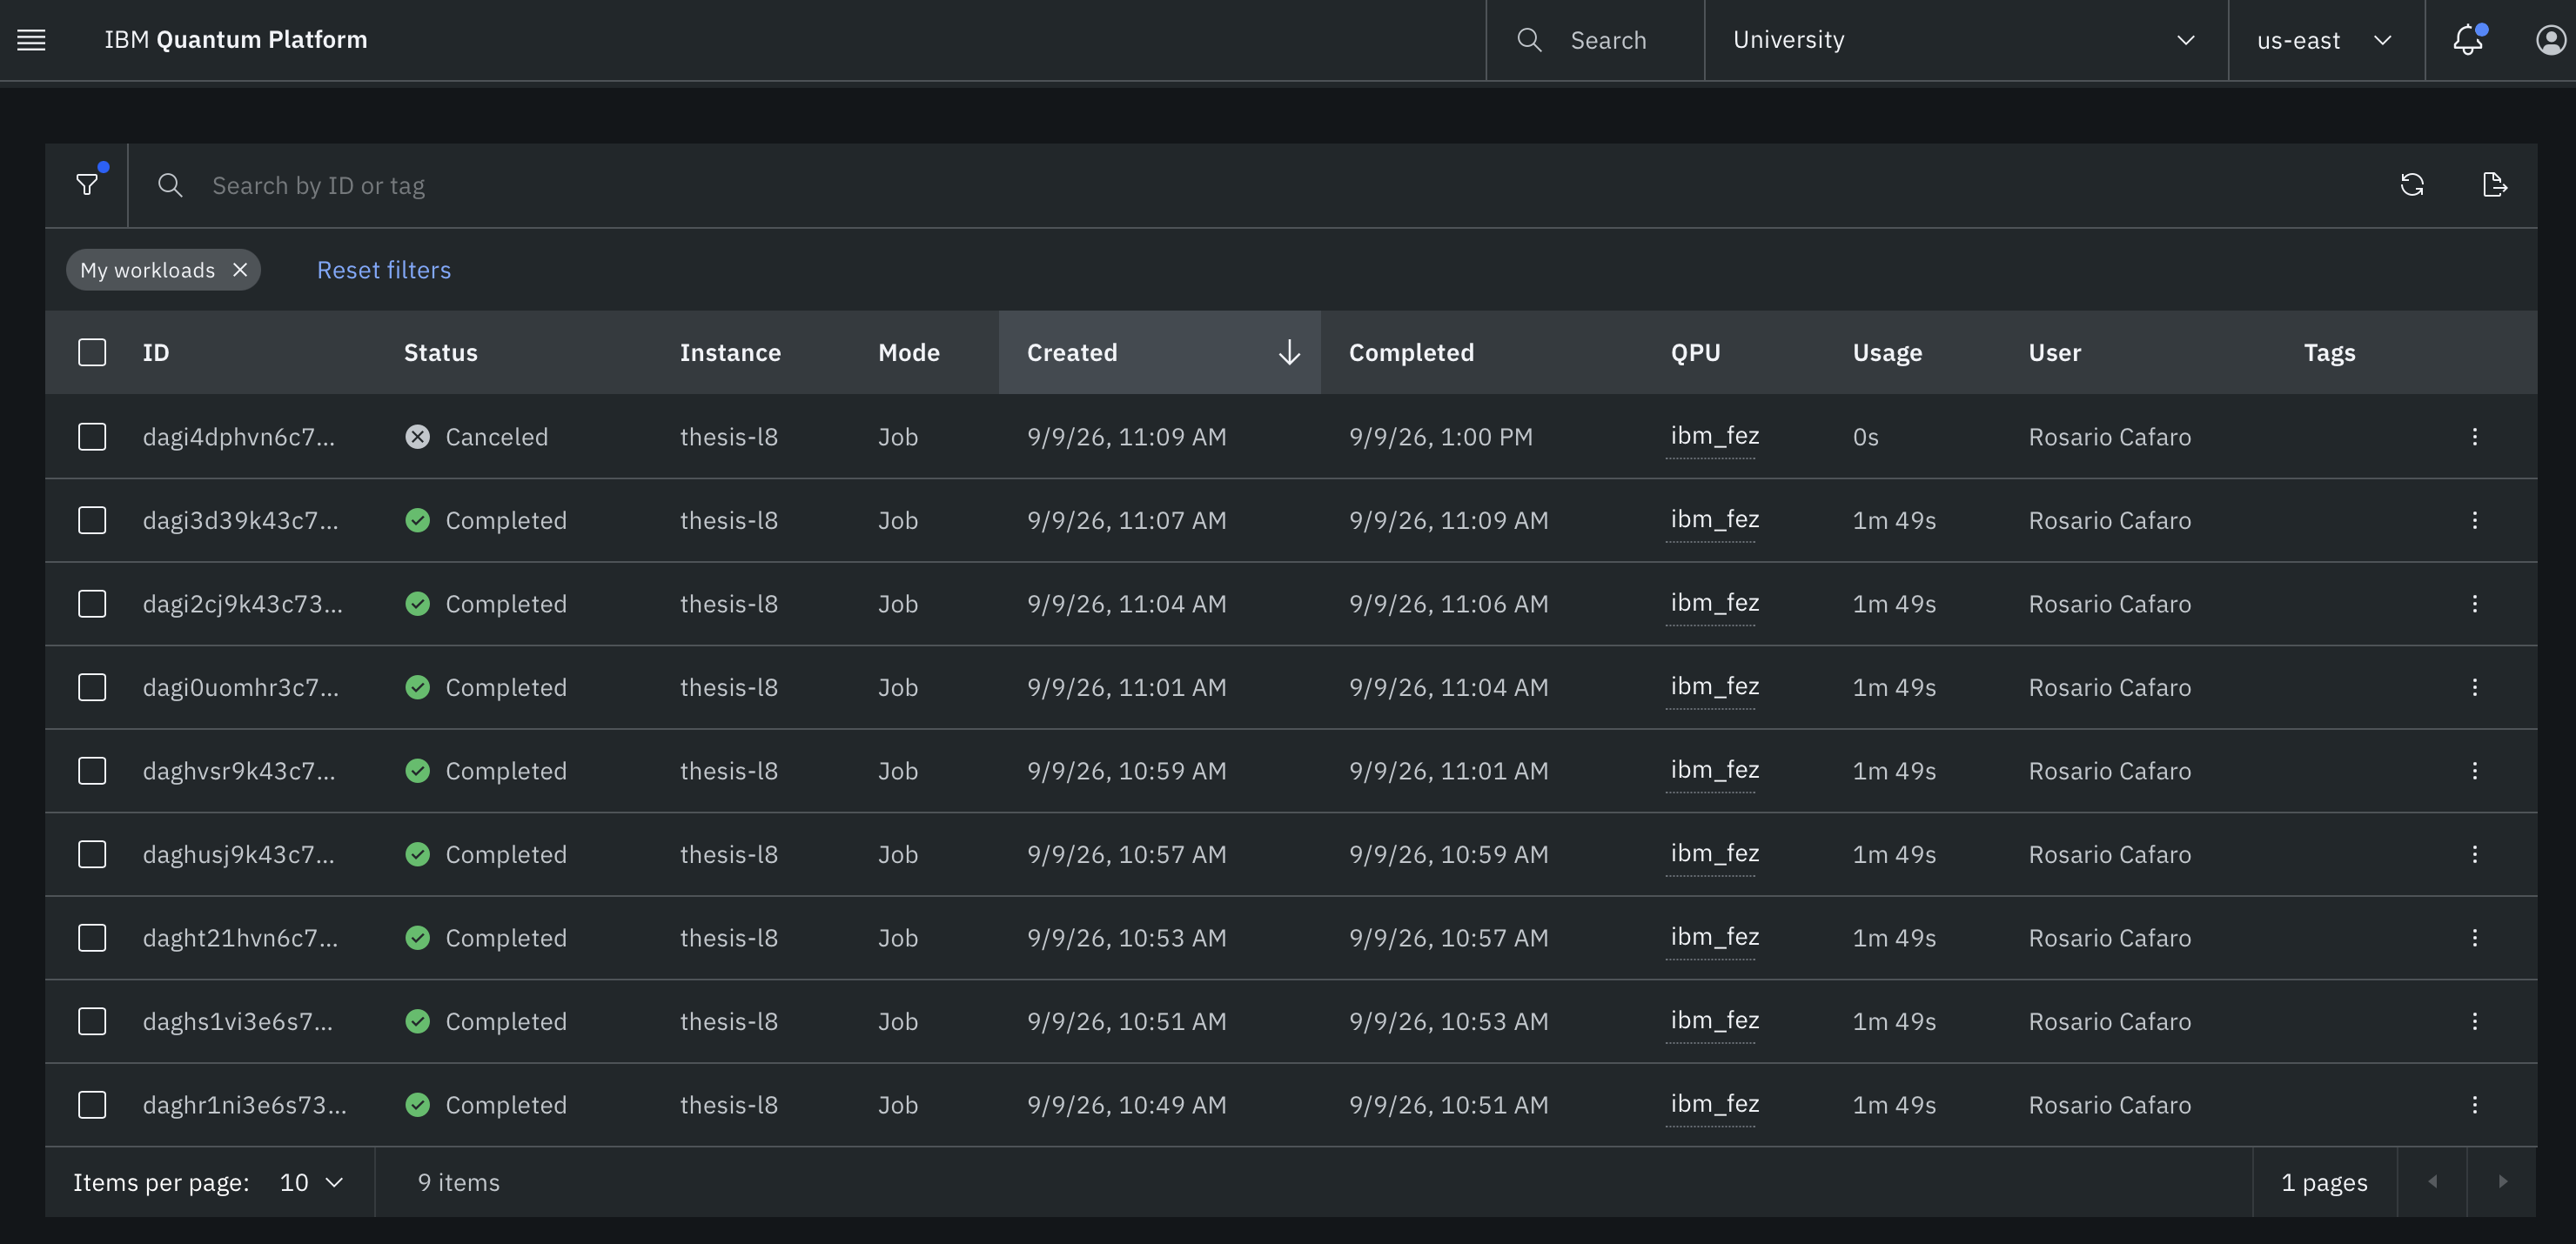
\includegraphics[width=\textwidth]{assets/IBM_quantum_platform_jobs.png}
        \caption{Pannello \textit{Workloads} di IBM Quantum Platform con i 9 job del tentativo di esecuzione su hardware reale: 8 completati in circa 1m49s ciascuno e 1 annullato (\textit{Canceled}, 0s di utilizzo) all'esaurimento della quota QPU del piano gratuito.}
        \label{fig:ibm_workloads_jobs}
    \end{figure}

    \item \textbf{Dimensione del training set per QSVC}: per calcolare la matrice di kernel, \texttt{FidelityQuantumKernel} invia un'unica chiamata al sampler, contenente una coppia di circuiti per ciascuna coppia di campioni di addestramento (una lista di PUB), per un totale di $O(N^2)$ circuiti logici sull'intero training set e non, come si potrebbe supporre, una chiamata o un job separato per coppia. Per training set fino ad alcune centinaia di campioni questo non pone problemi pratici anche in simulazione ideale (verificato per l'intero training set di Breast Cancer Wisconsin, 455 campioni, circa 103.000 coppie, con un picco di memoria di circa 785~MB in un'unica chiamata, misura coerente con il picco di memoria per coppia, circa 8KB, misurato empiricamente anche su \texttt{StatevectorSampler}).

    Per training set più ampi, però, il problema si presenta anche in simulazione ideale: il training set completo di Digits (circa 1.440 campioni, oltre un milione di coppie tra addestramento e predizione) ha esaurito la memoria disponibile del container Docker (limite di 8GB, Sezione~\ref{sec:struttura_progetto}) in un'unica chiamata, terminando il processo (\texttt{SIGKILL}, senza un'eccezione Python esplicita da intercettare) prima del completamento. In modalità \texttt{noisy\_simulation}, \texttt{AerSampler} ha inoltre un'impronta di memoria per coppia sostanzialmente più ripida di \texttt{StatevectorSampler}, al punto che un'unica chiamata con training set di alcune centinaia di campioni può esaurire la memoria disponibile prima di completare il calcolo, e su hardware reale una chiamata di queste dimensioni può eccedere i limiti per job del servizio IBM Quantum Platform.

    La soluzione adottata in tutti e tre i casi è il parametro \newline\texttt{max\_circuits\_per\_job} di \texttt{build\_qsvc}/\texttt{train\_and\_evaluate\_qsvc} (Sezioni~\ref{sec:impl_qsvc},~\ref{sec:impl_orchestrazione}), che suddivide la stessa, unica chiamata logica in più chiamate più piccole, riducendo il picco di memoria (o, per l'hardware reale, il numero di job necessari) senza ridurre il numero di coppie calcolate né alterare il risultato (verificato numericamente identico a quello di un'unica chiamata) e a fronte di un overhead di tempo trascurabile in simulazione (verificato empiricamente: tempo totale pressoché invariato tra chiamata singola e chunked). \texttt{config.py} definisce tre costanti distinte, ciascuna calibrata sul vincolo pratico specifico della propria modalità: \texttt{QSVC\_IDEAL\_MAX\_CIRCUITS\_PER\_JOB} (50.000 coppie per chiamata) per la simulazione ideale, dove il vincolo è il picco di memoria locale su un training set non sottocampionato; \newline\texttt{QSVC\_MAX\_CIRCUITS\_PER\_JOB} (100 coppie per chiamata) per \newline\texttt{noisy\_simulation}, dove il vincolo è ancora il picco di memoria locale, ma su \texttt{AerSampler}, che ha un'impronta per coppia sostanzialmente più ripida di \texttt{StatevectorSampler}; \newline\texttt{QSVC\_REAL\_HARDWARE\_MAX\_CIRCUITS\_PER\_JOB} (1.000 coppie per chiamata) per \texttt{real\_hardware}, dove il vincolo non è la memoria locale (l'esecuzione avviene sui server IBM) ma il numero di job e il relativo overhead per job, discusso nel punto precedente. Il training set per \newline\texttt{noisy\_simulation}/\texttt{real\_hardware} è inoltre già ridotto rispetto a quello completo (\texttt{HARDWARE\_TRAIN\_SAMPLE\_SIZE}/\texttt{HARDWARE\_TEST\_SAMPLE\_SIZE},
    \newline Sezione~\ref{sec:esecuzione_hardware_reale}) a scopo dimostrativo e per contenere i tempi di esecuzione. È un ulteriore restringimento di scala rispetto al "sottoinsieme rappresentativo di configurazioni" già discusso nella Sezione~\ref{sec:strategia_valutazione}, qui riferito al numero di campioni anziché al numero di configurazioni testate. Il sottocampionamento è realizzato tramite \texttt{stratified\_subsample} (\texttt{src/data/preprocessing.py}), che effettua un nuovo split stratificato anziché un semplice troncamento posizionale, in modo da preservare le proporzioni tra classi anche alle dimensioni ridotte richieste da queste due modalità.

    \item \textbf{Asimmetria nella ricerca degli iperparametri}: i modelli classici sono stati ottimizzati tramite ricerca a griglia con validazione incrociata stratificata a 5 fold (Tabella~\ref{tab:grid_search_classici}), mentre per QSVC e VQC è stata valutata una sola configurazione di feature map e ansatz per dataset (Tabella~\ref{tab:configurazione_completa}), integrata soltanto da alcune analisi mirate (sensitività al numero di componenti PCA per il QSVC su Digits, confronto tra COBYLA e SPSA per il VQC su Breast Cancer Wisconsin). Non sono stati esplorati sistematicamente il numero di ripetizioni, lo schema di entanglement, la struttura dell'ansatz né il parametro di regolarizzazione dell'SVM del QSVC, per ragioni di tempo e di risorse computazionali (il solo addestramento del QSVC su Digits richiede circa un'ora in simulazione ideale, Tabella~\ref{tab:risultati_digits_ideale}). Le conclusioni vanno quindi formulate con prudenza: i risultati mostrano che, nelle configurazioni quantistiche adottate, i modelli classici ottengono prestazioni migliori, ma non consentono di generalizzare tale esito a tutte le possibili configurazioni di QSVC e VQC, che con strutture di circuito o iperparametri diversi potrebbero comportarsi diversamente.

    \item \textbf{Interpretazioni non verificate direttamente}: i fenomeni richiamati per spiegare le prestazioni dei modelli quantistici, ossia i \textit{barren plateaus} per il VQC e la concentrazione del kernel per il QSVC, non sono stati misurati direttamente in questo lavoro (ad esempio tramite la varianza dei gradienti o degli elementi della matrice di kernel). Sono pertanto presentati come possibili interpretazioni coerenti con i risultati osservati e non come cause dimostrate; una loro verifica richiederebbe esperimenti dedicati.
\end{itemize}

\section{Considerazioni conclusive}
\label{sec:considerazioni_conclusive_implementazione}

In questo capitolo è stata descritta l'implementazione software del sistema presentato nel Capitolo~\ref{cap:architettura_sistema_metodologia}, incluso il codice sorgente dei moduli di acquisizione, preprocessing, codifica quantistica, addestramento, esecuzione e valutazione, nonché la configurazione completa dell'ambiente containerizzato basato su Docker. Sono stati riportati e analizzati i risultati sperimentali ottenuti applicando la metodologia descritta ai tre dataset reali selezionati (Breast Cancer Wisconsin, Wine, Digits), confrontando le performance dei modelli classici di baseline (Logistic Regression, SVM, Random Forest) con quelle dei modelli quantistici implementati (QSVC e VQC), in due dei tre ambienti di esecuzione progressivamente più realistici previsti dalla strategia di valutazione (simulazione ideale e simulazione con rumore); l'esecuzione su hardware quantistico reale, terzo ambiente previsto, non è stata completata per vincoli di quota e di costo riscontrati empiricamente e documentati nella Sezione~\ref{sec:limiti_studio}. È stata infine proposta una discussione critica dei risultati disponibili, alla luce sia dei principi teorici presentati nei Capitoli~\ref{cap:fondamenti_ml_classificazione_classica} e~\ref{cap:quantum_machine_learning}, sia dei limiti metodologici propri di questo lavoro.

Le conclusioni generali della tesi, che sintetizzano i risultati ottenuti in relazione agli obiettivi di ricerca enunciati nell'introduzione e delineano possibili direzioni di lavoro futuro, sono presentate nel capitolo conclusivo.
